\documentclass[10pt,dvipdfmx]{beamer}
\usepackage{pgfpages}
\usepackage{graphicx}
\usepackage{listings,jlisting}
\usepackage{fancybox}
\usepackage{hyperref}
\usepackage{multimedia}

%%%%%%%%%%%%%%%%%%%%%%%%%%%
%%% themes
%%%%%%%%%%%%%%%%%%%%%%%%%%%
\usetheme{Rochester}
%% no navigation bar
% default boxes Bergen Boadilla Madrid Pittsburgh Rochester
%% tree-like navigation bar
% Antibes JuanLesPins Montpellier
%% toc sidebar
% Berkeley PaloAlto Goettingen Marburg Hannover Berlin Ilmenau Dresden Darmstadt Frankfurt Singapore Szeged
%% Section and Subsection Tables
% Copenhagen Luebeck Malmoe Warsaw

%%%%%%%%%%%%%%%%%%%%%%%%%%%
%%% innerthemes
%%%%%%%%%%%%%%%%%%%%%%%%%%%
% \useinnertheme{circles}	% default circles rectangles rounded inmargin

%%%%%%%%%%%%%%%%%%%%%%%%%%%
%%% outerthemes
%%%%%%%%%%%%%%%%%%%%%%%%%%%
% outertheme
% \useoutertheme{default}	% default infolines miniframes smoothbars sidebar sprit shadow tree smoothtree


%%%%%%%%%%%%%%%%%%%%%%%%%%%
%%% colorthemes
%%%%%%%%%%%%%%%%%%%%%%%%%%%
\usecolortheme{seahorse}
%% special purpose
% default structure sidebartab 
%% complete 
% albatross beetle crane dove fly seagull 
%% inner
% lily orchid rose
%% outer
% whale seahorse dolphin

%%%%%%%%%%%%%%%%%%%%%%%%%%%
%%% fontthemes
%%%%%%%%%%%%%%%%%%%%%%%%%%%
\usefonttheme{serif}  
% default professionalfonts serif structurebold structureitalicserif structuresmallcapsserif

%%%%%%%%%%%%%%%%%%%%%%%%%%%
%%% generally useful beamer settings
%%%%%%%%%%%%%%%%%%%%%%%%%%%
% 
\AtBeginDvi{\special{pdf:tounicode EUC-UCS2}}
% do not show navigation
\setbeamertemplate{navigation symbols}{}
% show page numbers
\setbeamertemplate{footline}[frame number]


%%%%%%%%%%%%%%%%%%%%%%%%%%%
%%% define some colors for convenience
%%%%%%%%%%%%%%%%%%%%%%%%%%%

\newcommand{\mido}[1]{{\color{green}#1}}
\newcommand{\mura}[1]{{\color{purple}#1}}
\newcommand{\ore}[1]{{\color{orange}#1}}
\newcommand{\ao}[1]{{\color{blue}#1}}
\newcommand{\aka}[1]{{\color{red}#1}}

\setbeamercolor{syntax}{bg=cyan!20!white}
\setbeamercolor{example}{bg=yellow!20!white}
\setbeamercolor{output}{bg=white}

\newcommand{\resa}[1]{\ore{\textsl{$\rightarrow$ #1}}}
\newcommand{\res}[1]{\ore{\textsl{#1}}}

%%%%%%%%%%%%%%%%%%%%%%%%%%%
%%% how to typset code
%%%%%%%%%%%%%%%%%%%%%%%%%%%

\lstset{language = python,
numbers = left,
numberstyle = {\tiny \emph},
numbersep = 10pt,
breaklines = true,
breakindent = 40pt,
frame = tlRB,
frameround = ffft,
framesep = 3pt,
rulesep = 1pt,
rulecolor = {\color{black!20!white}},
rulesepcolor = {\color{black!20!white}},
flexiblecolumns = true,
keepspaces = true,
basicstyle = \ttfamily\small,
identifierstyle = ,
commentstyle = ,
stringstyle = ,
showstringspaces = false,
tabsize = 4,
escapechar=\@,
xrightmargin=3zw,
}

\title{Python \\ Speed Learning}
\institute{東京大学}
\author{田浦健次朗 \\ 電子情報工学科}
\date{}

\AtBeginSection[] % Do nothing for \section*
{
\begin{frame}
\frametitle{Contents}
\tableofcontents[currentsection,currentsubsection]
\end{frame}
}

\begin{document}
\maketitle

%%%%%%%%%%%%%%%%%%%%%%%%%%%%%%%%%% 
% \begin{frame}
% \frametitle{Contents}
% \tableofcontents
% \end{frame}

%%%%%%%%%%%%%%%%% 
% \begin{frame}[fragile]
% \frametitle{以下のスライド}
% 以下のスライドで,
% \begin{beamercolorbox}{syntax}
% 青地で囲まれているのは, 文法規則の説明
% \end{beamercolorbox}

% \begin{beamercolorbox}{example}
% 緑地で囲まれているのは, プログラム例
% \end{beamercolorbox}

% \begin{beamercolorbox}{output}
% 黄地で囲まれているのは, プログラムを実行した際の出力
% \end{beamercolorbox}
% \end{frame}

\begin{frame}
\tableofcontents
\end{frame}

%%%%%%%%%%%%%%%%% %%%%%%%%%%%%%%%%% 
\section{ロードマップ}
%%%%%%%%%%%%%%%%% %%%%%%%%%%%%%%%%% 

%%%%%%%%
\begin{frame}
\frametitle{プログラミング言語の習得}
\begin{itemize}
\item \ao{道具・概念を覚える}
  \begin{itemize}
  \item どのような場面でどの道具が必要になるか
  \item 関数(def),変数,繰り返し(for),条件分岐(if),リスト,配列,etc.
  \item $\approx$ 数学でどの問題にどの公式を使うか
  \item 言語が違っても共通部分大きい
  \end{itemize}

\item \ao{文法規則を理解する}
  \begin{itemize}
  \item 1文字でも間違ったら許してくれない
  \item 文法規則の表記法を理解し,「許されるプログラム」がわかるようになる
  \end{itemize}

\item \ao{実行規則を理解する}
  \begin{itemize}
  \item 「このプログラムを実行したら何が起きるのか」をしっかり理解する
  \item エラーがどうして起きたのか理解し,対処できるようになる
  \end{itemize}
\end{itemize}
\end{frame}


%%%%%%%%
\begin{frame}
\frametitle{Jupyter環境について最低限の事}
\begin{itemize}
\item 入力セルには,Pythonの\ao{「式」}または\ao{「文」}
(両者の区別は後ほど)を入力する
\item Shift + Enter でそのセルの中身を\ao{「実行」}する.
それが「式」だったら結果が表示される

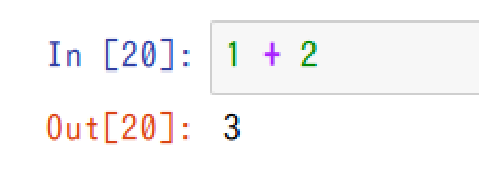
\includegraphics[width=0.3\textwidth]{out/pdf/img/cell_1_plus_2.pdf}

\item 一つのセルに複数の式(文)を書いてもよい.
結果が表示されるのは最後の式(文)だけ(実行は全て,されている).

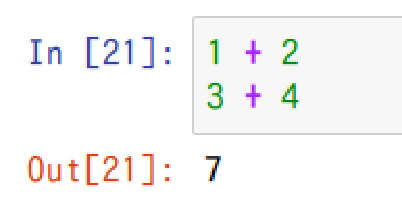
\includegraphics[width=0.3\textwidth]{out/pdf/img/cell_1_plus_2_3_plus_4.pdf}

\item 最初は,セルに1行入れてはその結果を見る,という使い方をするが,
徐々にひとつのセルに大きなプログラムを書いていくようになる
\end{itemize}
\end{frame}

%%%%%%%%
\begin{frame}[fragile]
\frametitle{このスライドでの入力とその結果の表記}
\begin{itemize}
\item このような実行例:

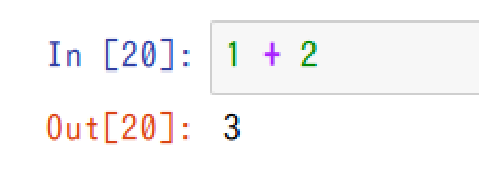
\includegraphics[width=0.3\textwidth]{out/pdf/img/cell_1_plus_2.pdf}

を,このスライドでは
\begin{lstlisting}
1 + 2
@\resa{3}@
\end{lstlisting}
のように表記
\end{itemize}
\end{frame}

%%%%%%%%%%%%%%%%% %%%%%%%%%%%%%%%%% 
\section{式}
%%%%%%%%%%%%%%%%% %%%%%%%%%%%%%%%%% 

%%%%%%%%%%%%%%%%%%%%
\begin{frame}[fragile]
\frametitle{式: 足し算,掛け算,累乗}
\begin{itemize}
\item 
\begin{lstlisting}
1 + 2
@\resa{3}@
\end{lstlisting}

\item 
\begin{lstlisting}
3 * 4
@\resa{12}@
\end{lstlisting}

\item 
\begin{lstlisting}
5 ** 6                  # @{\scriptsize $=5^6$}@
@\resa{15625}@
\end{lstlisting}

\item 
\begin{lstlisting}
7890 ** 1234            # @{\scriptsize $=7890^{1234}$ 巨大な数も軽々}@
@\resa{984060864275242374776504621337024479921780226636...}@
\end{lstlisting}
\end{itemize}
\end{frame}

%%%%%%%%%%%%%%%%%%%%
\iffalse
\begin{frame}[fragile]
\frametitle{式: 割り算には注意}
\begin{itemize}
\item 
\begin{lstlisting}
7.0 / 3.0
@\resa{2.3333333333333335}@
\end{lstlisting}

\item 
\begin{lstlisting}
7 / 3          # @{\scriptsize 整数/整数 は端数切り捨ての整数}@
@\resa{2}@
\end{lstlisting}

\item 
\begin{lstlisting}
7 / 3.0        # @{\scriptsize どちらかでも浮動小数点数ならば小数付きの割り算}@
@\resa{2.3333333333333335}@
\end{lstlisting}

\item 
\begin{lstlisting}
float(3)       # @{\scriptsize 整数を浮動小数点数に直す演算}@
@\resa{3.0}@
\end{lstlisting}

\item 
\begin{lstlisting}
7 / float(3)
@\resa{2.3333333333333335}@
\end{lstlisting}
\end{itemize}
\end{frame}
\fi

%%%%%%%%%%%%%%%%%%%%
\begin{frame}[fragile]
\frametitle{その他の式}
\begin{columns}
\begin{column}{0.5\textwidth}
\begin{itemize}
\item 余り
\begin{lstlisting}
13 @\ao{\tt \%}@ 7
@\resa{6}@
\end{lstlisting}

\item 等号は{\tt =}じゃなくて{\tt ==}
\begin{lstlisting}
1 @\ao{\tt ==}@ 2
@\resa{False}@
\end{lstlisting}

\item 大小比較
\begin{lstlisting}
3 @\ao{\tt <}@ 4
@\resa{True}@
\end{lstlisting}
\begin{lstlisting}
5 @\ao{\tt >=}@ 6
@\resa{False}@
\end{lstlisting}
\end{itemize}
\end{column} 
 
\begin{column}{0.5\textwidth}
\begin{itemize}
\item かつ,または
\begin{lstlisting}
7 <= 8 @\ao{\tt and}@ 9 == 9.0 
@\resa{True}@
\end{lstlisting}
\begin{lstlisting}
7 > 8 @\ao{\tt or}@ 9 != 9.0 
@\resa{False}@
\end{lstlisting}

\item 数学で慣れた記法
\begin{lstlisting}
10 < 11 < 12
@\resa{True}@
\end{lstlisting}

\item 実はTrueとは1 (Falseとは0)のこと
\begin{lstlisting}
True + 3
@\resa{4}@
\end{lstlisting}
\end{itemize}
\end{column}
\end{columns}
\end{frame}

%%%%%%%%%%%%%%%%% %%%%%%%%%%%%%%%%% 
\section{関数呼び出し}
%%%%%%%%%%%%%%%%% %%%%%%%%%%%%%%%%% 

%%%%%%%%%%%%%%%%%%%%
\begin{frame}[fragile]
\frametitle{関数}
いくつかの関数がPythonに組み込まれている
(一覧: \url{https://docs.python.jp/3.5/library/functions.html})

\begin{itemize}
\item
\begin{lstlisting}
abs(-2)
@\resa{2}@
\end{lstlisting}

\item
\begin{lstlisting}
float(3)
@\resa{3.0}@
\end{lstlisting}

\item
\begin{lstlisting}
int(4.5)
@\resa{4}@
\end{lstlisting}

\item
\begin{lstlisting}
min(10,20,30,40)
@\resa{10}@
\end{lstlisting}

\item
\begin{lstlisting}
(abs(-2) + float(3)) / max(50,60,70,80,90)
@\resa{0.05555555555555555}@
\end{lstlisting}

\end{itemize}
\end{frame}

%%%%%%%%%%%%%%%%%%%%
\begin{frame}[fragile]
\frametitle{print関数}
\begin{itemize}
\item 効果:
実行されると,$\langle$式$\rangle$を評価した結果をその場で表示する
\item 例:
\begin{lstlisting}
print(1 + 2)
print(7 / 3)
print(10 < 11 < 12)
@\resa{3}@
@\res{2.3333333333333335}@
@\res{True}@
\end{lstlisting}

\item 実行結果や途中経過を表示する道具

\end{itemize}
\end{frame}


%%%%%%%%%%%%%%%%% %%%%%%%%%%%%%%%%% 
\section{色々な機能の輸入(import)}
%%%%%%%%%%%%%%%%% %%%%%%%%%%%%%%%%% 

%%%%%%%%%%%%%%%%%%%%
\begin{frame}[fragile]
\frametitle{追加機能の輸入 (import)}
\begin{itemize}
\item 多くの関数は初めから組み込まれていない
\begin{lstlisting}
sin(1.0)
@\resa{(most recent call last):}@
@\res{  File "<stdin>", line 1, in <module>}@
@\res{\aka{name 'sin' is not defined}}@
\end{lstlisting}

\item 所望の機能(\ao{モジュール})を
「使いたい(\ao{import})」と宣言して初めて使える.
\begin{lstlisting}
@\ao{\tt import}@ math     # @{\scriptsize {\tt math}モジュールをimport}@
\end{lstlisting}
\begin{lstlisting}
@\ao{\tt math.sin}@(1.0)   # @{\scriptsize 「モジュール名.関数名」で目当ての関数が使える}@
@\resa{0.8414709848078965}@
\end{lstlisting}
\end{itemize}
\end{frame}

%%%%%%%%%%%%%%%%%%%%
\begin{frame}[fragile]
\frametitle{mathモジュールの頻出機能}
\begin{itemize}
\item $\sin$, $\cos$, $\tan$, $\pi$, $e$, $\exp$, $\log$, \ldots
\end{itemize}

\begin{columns}
\begin{column}{0.55\textwidth}
\begin{itemize}
\item
\begin{lstlisting}
math.@\ao{\tt sin}@(1.5)
@\resa{0.9974949866040544}@
\end{lstlisting}

\item
\begin{lstlisting}
math.@\ao{\tt cos}@(1.5)
@\resa{0.0707372016677029}@
\end{lstlisting}

\item
\begin{lstlisting}
math.@\ao{\tt pi}@
@\resa{3.141592653589793}@
\end{lstlisting}

\item
\begin{lstlisting}
math.sin(math.pi)
@\resa{1.2246467991473532e-16}@
\end{lstlisting}

\end{itemize}  
\end{column}
\begin{column}{0.55\textwidth}
\begin{itemize}
\item
\begin{lstlisting}
math.@\ao{\tt e}@
@\resa{2.718281828459045}@
\end{lstlisting}

\item
\begin{lstlisting}
math.@\ao{\tt exp}@(1.0)
@\resa{2.718281828459045}@
\end{lstlisting}

\item
\begin{lstlisting}
math.@\ao{\tt log}@(math.e)
@\resa{1.0}@
\end{lstlisting}

\item
\begin{lstlisting}
math.log(@\ao{\tt 81, 3}@)
@\resa{4.0}@
\end{lstlisting}
\end{itemize}
\end{column}
\end{columns}
\end{frame}

%%%%%%%%%%%%%%%%%%%%
\begin{frame}[fragile]
\frametitle{モジュールとの付き合い方}
\begin{itemize}
\item 文字通り無数の機能が「モジュール」として提供されている
\item 一部はPythonに常に付属している標準モジュール,
  一部は追加インストールが必要な外部モジュール
\item 本ゼミで使う,\ao{visual, matplotlib, numpy, scipy}
  などもすべて「(外部)モジュール」
\item 暗記は不可能.必要なモジュールを探し,その機能を調べられることが大事
  \begin{itemize}
  \item Google検索: \fbox{python math モジュール} とか
  \item Pythonの標準ライブラリ一覧: 
    \url{https://docs.python.jp/3.5/library/}
    % \url{http://docs.python.jp/2/library/}
  \end{itemize}
\end{itemize}
\end{frame}

%%%%%%%%%%%%%%%%%%%%
\begin{frame}[fragile]
\frametitle{Python環境内でモジュール・関数の機能を調べる方法}
\begin{itemize}
\item dir: モジュール内で定義されている名前の一覧
\begin{lstlisting}
@\ao{\tt dir}@(math)
@\resa{[ ... 'cos', 'cosh', .... ]}@
\end{lstlisting}

\item help:
\begin{lstlisting}
@\ao{\tt help}@(math.sin)
@\resa{Help on built-in function sin in module math:}@

    @\res{sin(x)}@

    @\res{Return the sine of x (measured in radians).}@
\end{lstlisting}

\begin{lstlisting}
@\ao{\tt help}@(math)
@\resa{mathモジュールに関する長〜い説明}@
\end{lstlisting}

\end{itemize}
\end{frame}

%%%%%%%%%%%%%%%%%%%%
\begin{frame}[fragile]
\frametitle{importの色々なスタイル}
\begin{itemize}
\item 正当:
\begin{lstlisting}
import math
math.sin(1.0)
\end{lstlisting}
\item 略記を定義:
\begin{lstlisting}
import numpy @\ao{\tt as}@ np
np.array([1,2,3])
\end{lstlisting}
\item モジュール名を省略$+$輸入する名前を限定
\begin{lstlisting}
from math import sin,cos,log
log(sin(1.0)**2 + cos(1.0)**2)
\end{lstlisting}
\item モジュール名を省略$+$全部の名前を輸入
\begin{lstlisting}
from visual import *
vector(1,2,3)
\end{lstlisting}
\end{itemize}
\end{frame}

%%%%%%%%%%%%%%%%% %%%%%%%%%%%%%%%%% 
\section{変数}
%%%%%%%%%%%%%%%%% %%%%%%%%%%%%%%%%% 

%%%%%%%%%%%%%%%%%%%%
\begin{frame}[fragile]
\frametitle{変数}
\begin{itemize}
\item これまでPythonで計算できる色々な式の形(四則や関数)を見た
\item ここまではいわば関数電卓レベル
\item プログラミング言語には,\ao{「変数」}というものがあり,
  計算の途中結果に名前を付けて(代入文),後の計算に利用できる
\item 例:
\begin{lstlisting}
@\ao{\tt c =}@ math.cos(1.0)   # @{\scriptsize 変数cに結果を格納(代入)}@
\end{lstlisting}
\begin{lstlisting}
c
@\resa{0.5403023058681398}@
\end{lstlisting}
\begin{lstlisting}
s = math.sin(1.0)
\end{lstlisting}
\begin{lstlisting}
@\ao{\tt c ** 2 + s ** 2}@    # @{\scriptsize 式に変数を使える}@
@\resa{1.0}@
\end{lstlisting}
\end{itemize}
\end{frame}

%%%%%%%%%%%%%%%%%%%%
\begin{frame}[fragile]
  \frametitle{変数の使いみち}
  $\approx$ 「値」に名前をつける
  \begin{itemize}
  \item 式を見やすくする
\begin{lstlisting}
3.1415926535 * 2.589 * 2.589
\end{lstlisting}
と書く代わりに    
\begin{lstlisting}
pi = 3.1415926535
r = 2.589
pi * r * r
\end{lstlisting}
\item 同じ式を2度書かなくてすむようにする
\item (主にfor文と組み合わせて) 変数の値を書き換えながら長い計算をする
\end{itemize}
\end{frame}
  
%%%%%%%%%%%%%%%%%%%%
\begin{frame}[fragile]
\frametitle{同じ変数に何度も代入できる}

\begin{itemize}
\item 同じ変数に何度代入しても良い.変数の値は「最後に代入された値」
\begin{lstlisting}
x = 3
x = 4
x
@\resa{4}@
\end{lstlisting}    
\item 代入の右辺にも変数を使って良い.
{\tt x = x + 1}などという,数学で見慣れない式に慣れるのも,
プログラミングの一部
\begin{lstlisting}
x = 4
x = x + 1   # x = 4 + 1
x
@\resa{5}@
\end{lstlisting}    
\end{itemize}
\end{frame}

%%%%%%%%%%%%%%%%% %%%%%%%%%%%%%%%%% 
\section{関数定義}
%%%%%%%%%%%%%%%%% %%%%%%%%%%%%%%%%% 

%%%%%%%%%%%%%%%%%%%%
\begin{frame}[fragile]
\frametitle{関数定義}
\begin{itemize}
\item 自分で新しい関数を定義し,使うことができる
  $\rightarrow$ プログラミングで最重要な概念
\item 例:
\begin{lstlisting}
@\ao{\tt def}@ f(x, y)@\ao{\tt :}@             # @{\scriptsize 関数fを定義}@
    @\ao{\tt return}@ x ** 2 + y ** 2
\end{lstlisting}
\begin{lstlisting}
f(3, 4)                  # @{\scriptsize x=3, y=4として関数fを使う(呼び出す)}@
@\resa{25}@
\end{lstlisting}
\end{itemize}
\end{frame}

%%%%%%%%%%%%%%%%%%%%
\begin{frame}[fragile]
\frametitle{関数本体に複数の文を並べても良い}
\begin{itemize}
\item 使い道: 長い式を一気に書くのではなく,
  変数などを使って適宜分解し,見やすくする
\item 
例: $a, b, c$から,
\[ \frac{-b + \sqrt{b^2 - 4 ac}}{2a} \]
を計算する関数{\tt solve\_q}:
\item 書き方1:
\begin{lstlisting}
def solve_q(a, b, c):
    return (-b + math.sqrt(b*b - 4*a*c)) / (2*a)
\end{lstlisting}
\item 書き方2:
\begin{lstlisting}
def solve_q(a, b, c):
    D = b * b - 4 * a * c
    return (-b + math.sqrt(D)) / (2 * a)
\end{lstlisting}
\end{itemize}
\end{frame}

%%%%%%%%%%%%%%%%%%%%
\begin{frame}[fragile]
  \frametitle{関数(定義)の使いみち}
  $\approx$ 「計算の過程」に名前をつける
  \begin{itemize}
  \item 式を見やすくする
\begin{lstlisting}
root = (-b + math.sqrt(b*b - 4*a*c)) / (2*a)      
\end{lstlisting}
の変わりに
\begin{lstlisting}
root = solve_q(a, b, c) # 2次方程式を解く
\end{lstlisting}
\item 同じ文・式・その組み合わせを2度書かなくてすむようにする
  \end{itemize}

  \ao{「変数」と「関数」を組み合わせて,
    意味がわかりやすく, 値の変更がしやすいプログラム}
\end{frame}
  
%%%%%%%%%%%%%%%%%%%%
\begin{frame}
\frametitle{プログラミング$\approx$関数の定義,関数の定義,\ldots}
\begin{itemize}
\item 難しい問題を解くプログラムは,多数の関数から成る
\item 簡単な関数を元に,それを部品として使って別の関数を作り,\ldots
\item 徐々に複雑な計算を組み立てていく
\end{itemize}

\end{frame}

%%%%%%%%%%%%%%%%%%%%
\begin{frame}[fragile]
\frametitle{関数呼び出し実行の規則}
\begin{itemize}
\item 関数呼び出し(e.g., {\tt f(a)})が実行されたら,
  {\tt f}の本体の文が上から順に実行される
\item その最中``{\tt return} $E$''が実行されたら$E$の結果が{\tt f(a)}の結果になる.{\tt f}の中にそれ以降文があっても実行されない.
\begin{lstlisting}
def f(x):
    return x + 1
    return x + 2  # 実行されない
\end{lstlisting}
\begin{lstlisting}
f(3)
@\resa{4}@
\end{lstlisting}
\end{itemize}
\end{frame}

%%%%%%%%%%%%%%%%%%%%
\begin{frame}[fragile]
\frametitle{関数定義の落とし穴}
\begin{itemize}
\item \aka{注:} {\tt return}が実行されることなく最後の文が終了すると,
\ao{\tt None}という謎な値になる
\begin{lstlisting}
def f(x):
    x + 1          # たぶんreturn文を書き忘れた
\end{lstlisting}
\begin{lstlisting}
f(4)    # 何も表示されない(実はNoneが「表示」されている)
\end{lstlisting}
\begin{lstlisting}
f(4) + 2           # None + 2 を実行することになり,エラー
@\resa{Traceback (most recent call last):}@
  @\res{File "<stdin>", line 1, in <module>}@
@\res{TypeError: \aka{unsupported operand type(s) for +: 'NoneType' and 'int'}}@
\end{lstlisting}
\end{itemize}
\end{frame}

%%%%%%%%%%%%%%%%%%%%
\begin{frame}
  \frametitle{プログラムは「文法」に沿って書かなくてはならない}
  \begin{itemize}
  \item 式, 変数, 関数呼び出し, \ldots などを習っていったとき,
    それらを正しく組み合わせられるよう,
    すべてがひとつの「文法」にしたがっているということを意識するとよい
  \item 英語の文型 文 $=$ S V O $|$ S V O C $|$ \ldots
    みたいなものだが, 英語と異なり\aka{「融通もないが例外もない」}
    $\rightarrow$ 意識して覚える必要・価値が高い
  \end{itemize}
\end{frame}

%%%%%%%%%%%%%%%%%%%%
\begin{frame}[fragile]
\frametitle{ここまでの文法(1)}
\begin{itemize}
\item セルに書いて良いもの
\begin{lstlisting}
@$\langle$@セル@$\rangle$@ ::=
@$\langle$@文@$\rangle$@
  @$\cdots$@
@$\langle$@文@$\rangle$@
\end{lstlisting}
\item (これまでに出てきた)文:
\begin{lstlisting}
@$\langle$@文@$\rangle$@ ::=
 @\ao{\tt return}@ @$\langle$@式@$\rangle$@    # return文
@$|$@ @$x$@ @\ao{\tt =}@ @$\langle$@式@$\rangle$@      # 代入文
@$|$@ @\ao{\tt import}@ @$m$@      # import文
@$|$@ @$\langle$@関数定義@$\rangle$@     # 実は関数定義も文
@$|$@ @$\langle$@式@$\rangle$@           # 実は式も文の一種
\end{lstlisting}
\end{itemize}
\end{frame}

%%%%%%%%%%%%%%%%%%%%
\begin{frame}[fragile]
\frametitle{関数定義の文法}
\begin{itemize}
\item 関数定義の本体には,「文」を任意個並べることができる
\begin{lstlisting}
@$\langle$関数定義$\rangle$@ ::=
@\ao{\tt def}@ @$f$@(@$x$@, @$y$@, @$\cdots$@):
    @$\langle$@文@$\rangle$@
     @$\cdots$@
    @$\langle$@文@$\rangle$@
\end{lstlisting}
\end{itemize}
\end{frame}

%%%%%%%%%%%%%%%%%%%%
\begin{frame}[fragile]
\frametitle{式の文法}
\begin{itemize}
\item (これまでに出てきた)式
\begin{lstlisting}
@$\langle$@式@$\rangle$@ ::=
 数                          # 1とか2.3とか
@$|$@ @$x$@                          # 変数の参照
@$|$@ @$\langle$@式@$\rangle$@ @$\langle$@演算子@$\rangle$@ @$\langle$@式@$\rangle$@        # 3 + 4とか
@$|$@ @$\langle$@演算子@$\rangle$@ @$\langle$@式@$\rangle$@             # -3 とか
@$|$@ @$\langle$@式@$\rangle$@ (@$\langle$@式@$\rangle$@, @$\langle$@式@$\rangle$@, @$\cdots$@)    # abs(-3)とか
@$|$@ @$\langle$@式@$\rangle$@ . @$x$@                  # math.sin とか
@$|$@ ( @$\langle$@式@$\rangle$@ )
\end{lstlisting}

\item 上記で$f$, $x$, $m$は変数名,関数名,モジュール名を表し,
文法上は\ao{「識別子」}と呼ばれる.
\item 識別子として許されるのは,
アルファベット(\ao{\tt A-Z}, \ao{\tt a-z}),
下線(\ao{\tt \_})および数字(\ao{\tt 0-9})の並び.
ただし先頭に数字は許されない.
\begin{itemize}
\item OK: {\tt x, y, sin, my\_func, Masahiro\_Tanaka\_19}
\item NG: {\tt x', 1st\_attempt, Masahiro Tanaka 19}
\end{itemize}
\end{itemize}
\end{frame}

%%%%%%%%%%%%%%%%%%%%
\begin{frame}[fragile]
\frametitle{文法の落とし穴(1)}
特に,他のプログラミング言語を知っている人は注意

\begin{itemize}
\item 式が長くても\aka{勝手に改行してはいけない}
\begin{lstlisting}
def f(x):
    return 3 * x * x * x * x
         + 4 * x * x * x
@\resa{File "<...>", line 3}@
    @\res{+ 4 * x * x * x}@
    @\res{$\hat{ }$}@
@\res{IndentationError: \aka{unexpected indent}}
\end{lstlisting}

\item {\tt def f(x)} のあとの,\aka{コロン({\tt :})を忘れない!}
\begin{lstlisting}
def f(x)
    return x ** 2

@\resa{File "<...>", line 1}@
    @\res{def f(x)}@
            @\res{$\hat{ }$}@
@\res{SyntaxError: \aka{invalid syntax}}@
\end{lstlisting}
\end{itemize}
\end{frame}

%%%%%%%%%%%%%%%%%%%%
\begin{frame}[fragile]
\frametitle{文法の落とし穴(2)}
\begin{itemize}

\item 関数本体は\aka{必ず字下げ}をする; 字下げされているところが関数内部
\begin{lstlisting}
def f(x):
    y = x + 1
    return y * y
    f(10)
\end{lstlisting}
{\tt f(10)}を実行しているつもりかも知れませんが,実行されません
  
\item 字下げは\aka{揃える}(字下げすればいいわけではない)
\begin{lstlisting}
def f(x):
    y = x + 1
      z = y * y
  return z ** 2
@\resa{File "<...>", line 3}@
    @\res{z = y * y}@
    @\res{$\hat{ }$}@
@\res{IndentationError: \aka{unexpected indent}}@
\end{lstlisting}

\item 今後も何かとこのパターン(\ao{コロン({\tt :})のあと字下げ})が出てきます

\end{itemize}
\end{frame}

%%%%%%%%%%%%%%%%% %%%%%%%%%%%%%%%%% 
\section{文}
%%%%%%%%%%%%%%%%% %%%%%%%%%%%%%%%%% 

%%%%%%%%%%%%%%%%%%%%
\begin{frame}[fragile]
\frametitle{さらなる文}

\begin{itemize}
\item これまでに学んだ文(主に代入文, return文)と式
  (算術式と組み込み関数)だけで書ける関数はたかが知れている
\item for文とif文を習うことで,かなりのことが書けるようになる

\begin{lstlisting}
@$\langle$@文@$\rangle$@ ::=
 return @$\langle$@式@$\rangle$@    # return文
@$|$@ @$x$@ = @$\langle$@式@$\rangle$@      # 代入文
@$|$@ import @$m$@      # import文
@$|$@ @$\langle$@関数定義@$\rangle$@     # 実は関数定義も文
@$|$@ @$\langle$@式@$\rangle$@           # 実は式も文の一種
@$|$@ @\ao{\tt for文}@
@$|$@ @\ao{\tt if文}@
\end{lstlisting}
\end{itemize}

% @$|$@ @\ao{\tt print文}@

\end{frame}

%%%%%%%%%%%%%%%%% %%%%%%%%%%%%%%%%% 
\subsection{繰り返し (for) 文}
%%%%%%%%%%%%%%%%% %%%%%%%%%%%%%%%%% 

%%%%%%%%%%%%%%%%%%%%
\begin{frame}[fragile]
\frametitle{繰り返し: for文の初歩}
\begin{itemize}
\item 文法: 本当はもう少し一般的だがまずは以下の形で:
\begin{lstlisting}
@\ao{\tt for}@ @$x$@ @\ao{\tt in range}@(@$E_0$@,@$E_1$@)@\ao{\tt :}@
    @$\langle$@文@$\rangle$@    
     @$\cdots$@
    @$\langle$@文@$\rangle$@    
\end{lstlisting}
\item $E_0$, $E_1$は任意の$\langle$式$\rangle$
\item 実行規則 ($\approx$ 本体を$E_1 - E_0$回繰り返す): 
  \begin{enumerate}
  \item $E_0$, $E_1$を計算(それぞれ$a$, $b$とする)
  \item $x = a$ として $\langle$文$\rangle$ $\cdots$ $\langle$文$\rangle$ を実行
  \item $x = a + 1$ として $\langle$文$\rangle$ $\cdots$ $\langle$文$\rangle$ を実行
  \item \ldots
  \item $x = b - 1$ として $\langle$文$\rangle$ $\cdots$ $\langle$文$\rangle$ を実行
  \end{enumerate}

\item $E_1$を省略可.{\tt range($E$)} $\equiv$ {\tt range(0, $E$)}
($\approx$ $E$回繰り返し)
\end{itemize}
\end{frame}

%%%%%%%%%%%%%%%%%%%%
\begin{frame}[fragile]
\frametitle{(あまり役に立たない) for文の例}
\begin{itemize}
\item 0から$n-1$まで表示
\begin{lstlisting}
def print_i(n):
    for i in range(n):
        print(i)

print_i(10)
@\resa{0}@
@\res{1}@
@\res{.}@
@\res{.}@
@\res{9}@
\end{lstlisting}

\item 注:
  \begin{itemize}
  \item {\tt print(..)}文は実行の途中経過を知る良い手段
  \item ただし大量に{\tt print}するとJupyter環境で
  \end{itemize}
\end{itemize}
\end{frame}

%%%%%%%%%%%%%%%%%%%%
\begin{frame}[fragile]
\frametitle{for文の中のfor文}
\begin{itemize}
\item for文自体が$\langle$文$\rangle$の一種で,
  for文の中には任意の$\langle$文$\rangle$が書けるのだから以下は正しい文
\begin{lstlisting}
def print_ij(n):
    for i in range(0, n):
        for j in range(10, 10 + n):
            print(i, j)

print_ij(3)
@\resa{0 10}@
@\res{0 11}@
@\res{0 12}@
@\res{1 10}@
@\res{1 11}@
@\res{1 12}@
@\res{2 10}@
@\res{2 11}@
@\res{2 12}@
\end{lstlisting}
\end{itemize}
\end{frame}

%%%%%%%%%%%%%%%%%%%%
\begin{frame}[fragile]
\frametitle{for文の例}
\begin{itemize}
\item $n$が与えられ,1から$n$までの和:
\[ \sum_{k=1}^n k^2 = 1^2 + \cdots + n^2 \]
を計算する
\begin{lstlisting}
def sum_k2(n):
    s = 0
    for k in range(1, n+1):
        s = s + k * k
    return s

sum_k2(10)
@\resa{385}@
\end{lstlisting}
\end{itemize}
\end{frame}

%%%%%%%%%%%%%%%%%%%% 
\begin{frame}[fragile]
\frametitle{for文の実行を理解する}
\begin{itemize}
\item 
\begin{lstlisting}
def sum_k2(n):
    s = 0
    for k in range(1, n+1):
        s = s + k * k
    return s
\end{lstlisting}
\item {\tt sum\_k(10)}実行の様子:
\begin{lstlisting}
s = 0
s = s + 1 * 1    # s = 1
s = s + 2 * 2    # s = 5
s = s + 3 * 3    # s = 14
   ...
s = s + 10 * 10  # s = 385
return s
\end{lstlisting}
\end{itemize}
\end{frame}

%%%%%%%%%%%%%%%%%%%%
\begin{frame}[fragile]
\frametitle{for文のあるある間違い}
\begin{itemize}
\item []
\begin{lstlisting}
def sum_k2(n):
    for k in range(1, n+1):
        s = s + k * k
    return s

sum_k2(3)
@\resa{}@
\end{lstlisting}
\begin{lstlisting}[basicstyle=\ttfamily\tiny]
---------------------------------------------------------------------------
UnboundLocalError                         Traceback (most recent call last)
<ipython-input-6-bb13f487ff09> in <module>()
@\aka{\tt ----> 1 sum\_k2(3)}@

<ipython-input-5-0e7b0b967ad8> in sum_k2(n)
      1 def sum_k2(n):
      2     for k in range(1, n+1):
@\aka{\tt ----> 3         s = s + k * k}@
      4     return s

@\aka{\tt UnboundLocalError: local variable 's' referenced before assignment}@
\end{lstlisting}
\end{itemize}
\end{frame}

%%%%%%%%%%%%%%%%%%%%
\begin{frame}[fragile]
  \frametitle{このエラーの起きた理由}
  \begin{enumerate}
  \item {\tt sum\_k2(3)}を実行しようとした
  \item $\rightarrow$
\begin{lstlisting}
for k in range(1, 4):
    s = s + k * k
\end{lstlisting}
\item $\rightarrow$
\begin{lstlisting}
    s = s + 1 * 1
\end{lstlisting}
\item $\rightarrow$ しかし(右辺の){\tt s}はまだ一度も代入されていない
  (値が不定)ためエラー
\begin{lstlisting}
    s = @\aka{s}@ + 1 * 1
\end{lstlisting}
\item 以下と同種のエラー
\begin{lstlisting}
def f(x):
    return y

f(3)
\end{lstlisting}
\end{enumerate}
\end{frame}

%%%%%%%%%%%%%%%%%%%%
\begin{frame}[fragile]
  \frametitle{教訓 (エラーとの付き合い方)}
  \begin{itemize}
  \item \ao{プログラムの実行規則はいつも同じ.} 普通に実行していって,
    ありえない(これ以上進めない)状況に遭遇するとエラーになる
  \item エラーの記録から以下を読み取る
    \begin{itemize}
    \item エラーの種類・説明(最後の行)
\begin{lstlisting}[basicstyle=\ttfamily\scriptsize]
UnboundLocalError: local variable 's' referenced before assignment
(局所変数's'が代入される前に参照された)
\end{lstlisting}
    \item どこでエラーが起きているか (最後の{\tt ---->})
\begin{lstlisting}
----> 3         s = s + k * k        
\end{lstlisting}
    \item そこに至るまでの関数呼び出しの履歴
\begin{lstlisting}
----> 1 sum_k2(3)      
\end{lstlisting}
\end{itemize}
\item $\Rightarrow$ {\tt sum\_k2(3)}を実行中, その中のfor文を実行中,
  その中の{\tt s = s + k * k}を実行しようとしたところで,
  代入されたことがなかった{\tt s}を参照しようとした
\end{itemize}
\end{frame}

%%%%%%%%%%%%%%%%%%%%
\begin{frame}[fragile]
  \frametitle{教訓 (for文のあるあるなエラー)}
  \begin{itemize}
  \item for文の中である変数(今回の{\tt s})を,
    自分自身で更新する({\tt s = ... s ... })ことはよくある
  \item そういう時, \aka{for文に先立って}
    その変数に代入しておかないといけないのでは?
    と反射的に思えるように
    \begin{itemize}
\item (多分)NG:
\begin{lstlisting}
for ...
    s = ... s ...  
\end{lstlisting}
\item 必要:
\begin{lstlisting}
s = ...    
for ...
    s = ... s ...  
\end{lstlisting}
\end{itemize}
\end{itemize}
\end{frame}

%%%%%%%%%%%%%%%%%%%%
\begin{frame}[fragile]
\frametitle{数式からfor文への翻訳作業例(1)}
\begin{itemize}
\item 方法1: 手計算する自分の姿をイメージ: 
\[ 1^2 + 2^2 + \cdots + n^2 \]
\begin{eqnarray*}
s & = & 0 \\
s & = & s + 1^2 (= 1) \\
s & = & s + 2^2 (= 5) \\
s & = & s + 3^2 (= 14) \\
  &   &  \cdots  \\
s & = & s + n^2 \\
\end{eqnarray*}
($\rightarrow$ $k$を1から$n$まで動かして$s = s + k^2$を繰り返すと見抜く)
\begin{lstlisting}
s = 0
for k in range(1, n+1):
    s = s + k * k  
\end{lstlisting}
\end{itemize}
\end{frame}

%%%%%%%%%%%%%%%%%%%%
\begin{frame}[fragile]
\frametitle{数式からfor文への翻訳作業例(2)}
\begin{itemize}
\item ややこしい場合は,漸化式を元にするのはいい方法.一般に,
\begin{lstlisting}
s = @$c$@
for i in range(0, @$n$@):
    s = @$f$@(s) 
\end{lstlisting}
の終了後の{\tt s}は,
\[
\left\{
\begin{array}{rcl}
s_0 & = & c,  \\
s_{i+1} & = & f(s_i)
\end{array}
\right.
\]
という数列の,$s_n$を保持している.

\item 従って逆に,求めたいものを上記の漸化式に書きなおせば,
for文への翻訳は機械的:
\end{itemize}
\end{frame}

%%%%%%%%%%%%%%%%%%%%
\begin{frame}[fragile]
\frametitle{数式からfor文への翻訳作業例(2')}
\begin{itemize}
\item 例:
\[ s_n = 1^2 + 2^2 + \cdots + n^2 \]
$\rightarrow$ 漸化式に翻訳
\begin{eqnarray*}
s_0 & = & 0  \\
s_{i+1} & = & s_i + (i+1)^2 
\end{eqnarray*}
$\rightarrow$ プログラムに翻訳
\begin{lstlisting}
s = 0
for i in range(0, n):
    s = s + (i + 1) ** 2
\end{lstlisting}
\end{itemize}
\end{frame}


%%%%%%%%%%%%%%%%% %%%%%%%%%%%%%%%%% 
\subsection{条件分岐 (if) 文}
%%%%%%%%%%%%%%%%% %%%%%%%%%%%%%%%%% 

%%%%%%%%%%%%%%%%%%%%
\begin{frame}[fragile]
\frametitle{条件分岐: if文}
\begin{itemize}
\item 文法:
\begin{lstlisting}
if @$\langle$@式@$\rangle$@:
   @$\langle$@文@$\rangle$@
    @$\cdots$@
   @$\langle$@文@$\rangle$@
else:
   @$\langle$@文@$\rangle$@
    @$\cdots$@
   @$\langle$@文@$\rangle$@
\end{lstlisting}
\item 実行規則:
  \begin{enumerate}
  \item $\langle$式$\rangle$を評価
  \item 結果が「真」であれば,{\tt else:}以前の
    $\langle$文$\rangle$ $\cdots$
    $\langle$文$\rangle$を,そうでなければ{\tt else:}以降
    の$\langle$文$\rangle$ $\cdots$
    $\langle$文$\rangle$を順に実行
  \end{enumerate}
\item {\tt else:}部分は省略可(何もしない)
\end{itemize}
\end{frame}


%%%%%%%%%%%%%%%%%%%%
\begin{frame}[fragile]
\frametitle{if文の例(1)}
\begin{itemize}
\item 小さい方を返す

\begin{lstlisting}
def smaller(x, y):
    if x < y:
        return x
    else:
        return y
\end{lstlisting}

\item 3の倍数と3のつく数を表示する
\begin{lstlisting}
def nabeatsu():
    for i in range(50):
        if i % 3 == 0 or 30 <= i < 40:
            print(i)
\end{lstlisting}
\end{itemize}
\end{frame}

%%%%%%%%%%%%%%%%%%%%
\begin{frame}[fragile]
\frametitle{if文の例(2)}
\begin{itemize}
\item 素数を判定($n$が素数$\iff$ $2, \cdots , (n - 1)$のどれでも割り切れない)
\begin{lstlisting}
def prime(n):
    if n == 1:
        return 0
    for i in range(2, n):
        if n % i == 0:
            return 0  # 割り切れたから素数じゃない
    return 1
\end{lstlisting}

\item $n-1$までの素数を数える
\begin{lstlisting}
def count_prime(n):
    c = 0
    for i in range(1, n):
        if prime(i):
            c = c + 1
    return c
\end{lstlisting}

\item {\tt if}の$\langle$式$\rangle$部では,
  0以外の全ての数が「真」とみなされる

\end{itemize}
\end{frame}


%%%%%%%%%%%%%%%%%%%%
\begin{frame}[fragile]
\frametitle{3つ以上に分岐するif文}
\begin{itemize}
\item 文法:
\begin{lstlisting}
if @$\langle$@式@$\rangle$@:
    @$\cdots$@
elif @$\langle$@式@$\rangle$@:
    @$\cdots$@
elif @$\langle$@式@$\rangle$@:
    @$\cdots$@
@$\cdots$@
else:
    @$\cdots$@
\end{lstlisting}
\item {\tt elif} ({\tt else if}の省略形だと思えば良い)をいくつでも書ける
\item ここでも{\tt else:}部分は省略可(何もしない)
\end{itemize}
\end{frame}


%%%%%%%%%%%%%%%%%%%%
\begin{frame}[fragile]
\frametitle{{\tt break文, continue文, pass文}}

\begin{itemize}
\item 概念的に大したことはないが一応

\begin{lstlisting}
@$\langle$@文@$\rangle$@ ::=
 return @$\langle$@式@$\rangle$@    # return文
@$|$@ @$x$@ = @$\langle$@式@$\rangle$@      # 代入文
@$|$@ import @$m$@      # import文
@$|$@ @$\langle$@関数定義@$\rangle$@     # 実は関数定義も文
@$|$@ @$\langle$@式@$\rangle$@           # 実は式も文の一種
@$|$@ for文
@$|$@ if文
@$|$@ @\ao{\tt break}@
@$|$@ @\ao{\tt continue}@
@$|$@ @\ao{\tt pass}@
\end{lstlisting}
\end{itemize}
% @$|$@ @\ao{\tt print文}@

\end{frame}


%%%%%%%%%%%%%%%%%%%%
\begin{frame}[fragile]
\frametitle{{\tt break, continue, pass}}

\begin{columns}
\begin{column}{0.55\textwidth}
\begin{itemize}
\item {\tt break} $\rightarrow$ for文(全体)をそこでやめる
\begin{lstlisting}
for i in range(1, 8):
    if i % 3 == 0:
        @{\tt break}@
    print i
@\resa{1}@
@\res{2}@
\end{lstlisting}
\end{itemize}
\end{column}


\begin{column}{0.55\textwidth}
\begin{itemize}
\item {\tt continue} $\rightarrow$ for文の「現在の繰り返し」をそこでやめる
\begin{lstlisting}
for i in range(1, 8):
    if i % 3 == 0:
        @{\tt continue}@
    print(i)
@\resa{1}@
@\res{2}@
@\res{4}@
@\res{5}@
@\res{7}@
\end{lstlisting}
\end{itemize}

\end{column}
\end{columns}
\end{frame}

%%%%%%%%%%%%%%%%%%%%%%%%%%%%%%%%%%%%%%%%


%%%%%%%%%%%%%%%%% %%%%%%%%%%%%%%%%% 
\section{より複雑なデータ}
%%%%%%%%%%%%%%%%% %%%%%%%%%%%%%%%%% 

%%%%%%%%%%%%%%%%% 
\begin{frame}[fragile]
\frametitle{より複雑なデータ}
\begin{itemize}
\item これまで, 式の結果として得られる値は基本的には,
ひとつの数値だけだった
\begin{itemize}
\item 2次元ベクトルなら変数二つ,3次元ベクトルなら変数三つ,\ldots
100次元なら\ldots ?
\end{itemize}

\item 実用的なプログラム(e.g., ベクトル, 行列, 四角, 丸, 果物,
自動車 \ldots)のためには, より複雑な値, 
特に「複数の値を組み合わせた値」が必要

\item Pythonに備わる,複合 (compound) データ
\begin{itemize}
\item リスト
\item タプル
\item 文字列
\item 辞書(説明せず)
\item オブジェクト
\end{itemize}
\end{itemize}

\end{frame}


%%%%%%%%%%%%%%%%% 
\begin{frame}
\frametitle{以降のroadmap}

\begin{center}
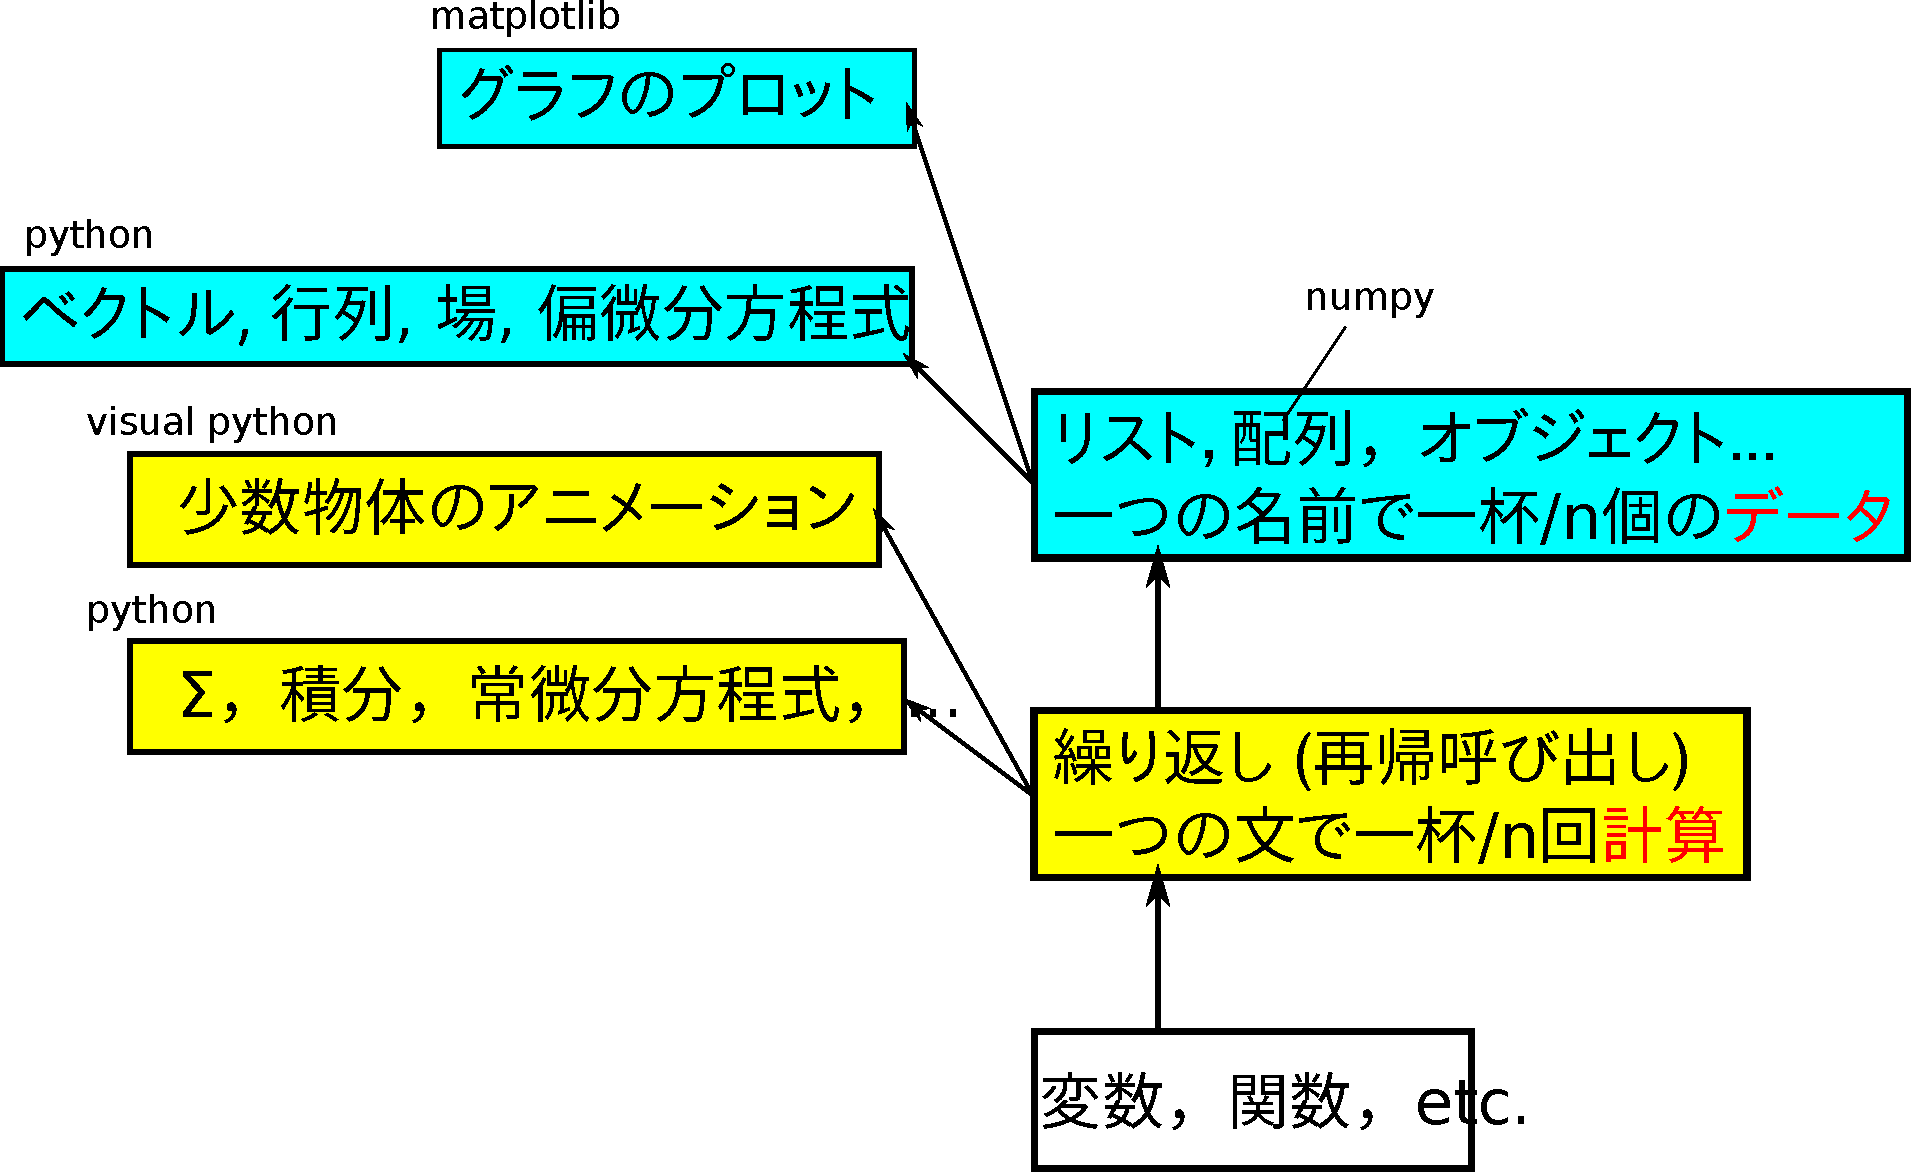
\includegraphics[width=1.0\textwidth]{out/pdf/svg/roadmap.pdf}
\end{center}

\end{frame}


%%%%%%%%%%%%%%%%% %%%%%%%%%%%%%%%%% 
\section{リスト}
%%%%%%%%%%%%%%%%% %%%%%%%%%%%%%%%%% 

%%%%%%%%%%%%%%%%% 
\begin{frame}[fragile]
\frametitle{リスト}
\begin{itemize}
\item 文法 (式の一種):
\begin{lstlisting}
@$\langle$@式@$\rangle$@ ::=
 数
@$|$@ @$x$@
@$|$@ @$\langle$@式@$\rangle$@ @$\langle$@演算子@$\rangle$@ @$\langle$@式@$\rangle$@
    @$\cdots$@
@$|$@ @\ao{\tt [ 式, 式, \ldots, 式 ]}@ # リストを作る
@$|$@ @\ao{\tt 式[式]}@             # 要素をアクセス
\end{lstlisting}

\item {\tt [ $E_0, E_1, \cdots, E_{n-1}$ ]} : $E_0, \cdots, E_{n-1}$ (それぞれを計算した結果)を一本に束ねた値(リスト)
\item {\tt $L[i]$} : $L$ (を計算した結果のリスト) の $i$ (を計算した結果)番目の要素 (ただし最初の要素は「0番目」)
\end{itemize}
\end{frame}

%%%%%%%%%%%%%%%%% 
\begin{frame}[fragile]
\frametitle{リスト : 例}
\begin{itemize}
\item []
\begin{lstlisting}
import math
x = 20
a = @\ao{\tt [ 1, 1+2, math.cos(0.0), x ]}@
\end{lstlisting}
\begin{lstlisting}
a
@\resa{[1, 3, 1.0, 20]}@
\end{lstlisting}
\begin{lstlisting}
@\ao{\tt len}@(a)
@\resa{4}@
\end{lstlisting}
\begin{lstlisting}
a@\ao{\tt [1]}@
@\resa{3}@
\end{lstlisting}
\begin{lstlisting}
a @\ao{\tt +}@ [1.2, 3.4]
@\resa{[1, 3, 1.0, 20, 1.2, 3.4]}@
\end{lstlisting}
\begin{lstlisting}
[ a, a, a ]
@\resa{[[1, 3, 1.0, 20], [1, 3, 1.0, 20], [1, 3, 1.0, 20]]}@
\end{lstlisting}
\end{itemize}
\end{frame}

%%%%%%%%%%%%%%%%% 
\begin{frame}[fragile]
\frametitle{リスト : 確認事項}
\begin{itemize}
\item リストも数値と同様, 「値」の一種に過ぎない
\item 数値と同様, 変数に代入したり, 他の関数へ渡したりできる
\item リストを受け取る関数, リストを返す関数, も書ける
\item \ao{「値の種類」が増えたこと以外, 新しいことはない}
\begin{lstlisting}
def f(l):
  return l[0]

f([1,2,3]) 
@\resa{1}@
\end{lstlisting}
\end{itemize}
\end{frame}


%%%%%%%%%%%%%%%%% 
\begin{frame}[fragile]
\frametitle{リストの書き換え}
リストには, 値を追加・削除したり, 書き換えたりすることができる
\begin{itemize}
\item []
\begin{lstlisting}
a = [ 2, 3, 5 ]
a@\ao{\tt .append}@(7) # 末尾に追加
a
@\resa{[2, 3, 5, 7]}@
\end{lstlisting}
\item []
ので, 繰り返し(for)を使ってとても長いリストを作ることもできる
\begin{lstlisting}
a = []
for i in range(0, 10000):
  a.append(i)
a
@\resa{[0, 1, 2, ..., 9999]}@  
\end{lstlisting}
\end{itemize}
\end{frame}

%%%%%%%%%%%%%%%%% 
\begin{frame}[fragile]
\frametitle{リストの書き換え}
リストには, 値を追加・削除したり, 書き換えたりすることができる
\begin{itemize}
\item [] (書き換え)
\begin{lstlisting}
a[2] = 50
a
@\resa{[2, 3, 50, 7]}@
\end{lstlisting}
\item [] (削除)
\begin{lstlisting}
@\ao{\tt del}@ a[1]    # a[1]を削除. 以降の要素は前にずれる
a
@\resa{[2, 50, 7]}@
\end{lstlisting}
\end{itemize}
\end{frame}


%%%%%%%%%%%%%%%%% 
\begin{frame}[fragile]
\frametitle{リストの書き換え}
リストには, 値を追加・削除したり, 書き換えたりすることができる
\begin{itemize}
\item []
\begin{lstlisting}
b = [ a, a, a ]
b
[[2, 50, 7], [2, 50, 7], [2, 50, 7]]
\end{lstlisting}
\begin{lstlisting}
a[2] = 30   # 注目
b
[[2, @\ao{\tt 30}@, 7], [2, @\ao{\tt 30}@, 7], [2, @\ao{\tt 30}@, 7]]
\end{lstlisting}
\begin{lstlisting}
@\ao{\tt dir}@(a)      # リストにできることは?
@\resa{[ ... 'append', 'count', 'extend', 'index', 'insert', 'pop', 'remove', 'reverse', 'sort']}@
@\ao{help(a.reverse)}@
@\res{ ...}@
\end{lstlisting}
\end{itemize}
\end{frame}


%%%%%%%%%%%%%%%%% 
\begin{frame}[fragile]
\frametitle{リスト内包表記}
\begin{itemize}
\item for文で計算した結果を「一発で」リストにする強力な記法
\item 覚えなくても問題ないが,覚えると賢くなった気がする
\item 文法:
\begin{lstlisting}
@$\langle$@式@$\rangle$@ ::=
    @$\cdots$@
@$|$@ @\ao{\tt [ 式 for 名前 in range(式, 式) ]}@
\end{lstlisting}

\item for文同様,本当はもっと一般的(後述).

\item 意味: {\tt [ $E$ for 名前 in range(式, 式) ]}は,あたかも
\begin{lstlisting}
for 名前 in range(式, 式): 
  @$E$@
\end{lstlisting}
実行し,$E$を計算した結果を全てリストにする

\item 例を見たほうが早い
\end{itemize}
\end{frame}


%%%%%%%%%%%%%%%%% 
\begin{frame}[fragile]
\frametitle{リスト内包表記 : 例}
\begin{itemize}
\item []
\begin{lstlisting}
[ x * x for x in range(0, 5) ]
@\resa{[0, 1, 4, 9, 16]}@
\end{lstlisting}

\item []
\begin{lstlisting}
sum([ x * x for x in range(0, 5) ])
@\resa{30}@
\end{lstlisting}
({\tt sum}はリストの和を取る関数)

% \item 
% \begin{lstlisting}
% >>> X = [ a + (b - a) * i / float(n) for i in range(0, 100000) ]
% >>> sum([ f(x) * (b - a) / float(n) for x in X ]
% \end{lstlisting}
\end{itemize}

それぞれ以下のようにしても同じことだがずっと簡潔
\begin{itemize}
\item []
\begin{lstlisting}
s = []
for x in range(0, 5):
  s.append(x * x)
\end{lstlisting}

\item []
\begin{lstlisting}
s = []
for x in range(0, 5):
  s += x * x
\end{lstlisting}
(注: {\tt s += $E$} は {\tt s = s + $E$}と同じ意味)

% \item 
% \begin{lstlisting}
% >>> X = [ a + (b - a) * i / float(n) for i in range(0, 100000) ]
% >>> sum([ f(x) * (b - a) / float(n) for x in X ]
% \end{lstlisting}
\end{itemize}
\end{frame}


%%%%%%%%%%%%%%%%% %%%%%%%%%%%%%%%%% 
\section{タプル (組)}
%%%%%%%%%%%%%%%%% %%%%%%%%%%%%%%%%% 

%%%%%%%%%%%%%%%%% 
\begin{frame}[fragile]
\frametitle{タプル}
\begin{itemize}
\item 文法:
\begin{lstlisting}
@$\langle$@式@$\rangle$@ ::=
    @$\cdots$@
@$|$@ @\ao{\tt 式, 式, \ldots, 式}@
\end{lstlisting}
混乱しないよう, 習慣として括弧をつける
\begin{lstlisting}
@\ao{\tt (式, 式, \ldots, 式)}
\end{lstlisting}

\item 意味: 各式を計算した結果を一本に束ねた値
\item リストとほとんど同じ! 実際, 以下はリストと同様に使える
  \begin{itemize}
  \item {\tt len(\ldots)} (要素数)
  \item {\tt \ldots[\ldots]} (指定要素)
  \item {\tt \ldots\ + \ldots} (連結)
  \end{itemize}

\end{itemize}
\end{frame}

%%%%%%%%%%%%%%%%% 
\begin{frame}[fragile]
\frametitle{タプルとリストの違い}
\begin{itemize}
\item タプルは, 一度作ったら要素の追加, 削除, 変更などはできない
\item 
\begin{lstlisting}
a = (1.1, 2.2, 3.3)
a.append(4.4) # @\aka{\tt NG}@
del a[1]      # @\aka{\tt NG}@
a[1] = 22     # @\aka{\tt NG}@
a = (4.4, 5.5) # OK
a = a + (6.6, 7.7) # OK
\end{lstlisting}
\item 最後の2つは, 変数を書き換えているのであってタプルを書き換えている
  のではない
\item タプル$\approx$リストを不便にしただけ?
\end{itemize}
\end{frame}

%%%%%%%%%%%%%%%%% 
\begin{frame}[fragile]
\frametitle{タプルの典型的使用場面}
\begin{itemize}
\item 二つ以上の値を一度に返す関数を手軽に書く
\begin{lstlisting}
def polar(x, y):
    r = sqrt(x * x + y * y)
    theta = atan2(y, x)
    return (r,theta)
\end{lstlisting}
\item 注: {\small 
「二つの値を返す」という言い方はあまり正しくない.
\ao{二つの値を組にした一つの値($=$タプル)}が作れる}

\item 変数に結果を受け取るときもこんなふうに書ける
\begin{lstlisting}
r,theta = polor(3, 4)
\end{lstlisting}

\item 実はこれでも「なぜリストだけじゃダメ?」の答えにはなっていないが
  \begin{itemize}
  \item これもOKだったりするので\ldots
\begin{lstlisting}
[a0,a1,a2] = range(3,6)  # a0=3, a1=4, a2=5
\end{lstlisting}
\end{itemize}

\end{itemize}
\end{frame}


%%%%%%%%%%%%%%%%% %%%%%%%%%%%%%%%%% 
\section{文字列}
%%%%%%%%%%%%%%%%% %%%%%%%%%%%%%%%%% 

%%%%%%%%%%%%%%%%% 
\begin{frame}[fragile]
\frametitle{文字列}
\begin{itemize}
\item 文法:
\begin{lstlisting}
@$\langle$@式@$\rangle$@ ::=
    @$\cdots$@
@$|$@   @\ao{\tt "文字文字 \ldots 文字"}@
@$|$@   @\ao{\tt '文字文字 \ldots 文字'}@
@$|$@ @\ao{\tt """文字文字 \ldots 文字"""}@
@$|$@ @\ao{\tt '''文字文字 \ldots 文字'''}@
\end{lstlisting}

\item どれもほとんど同じ意味. なぜ色々ある?
  \begin{itemize}
  \item 文字列中に{\tt "}を含めたければ, {\tt '}が便利. 逆もまた然り
    \begin{itemize}
    \item \ao{\tt a = '"Hi!", said he.'}
    \item \ao{\tt b = "Obama's speech"}
    \end{itemize}
  \item 3連打({\tt """}, {\tt '''})は, 改行を含んでも良い
  \end{itemize}

\item そして, できる操作はまたしてもリストやタプルとそっくり
  \begin{itemize}
  \item {\tt len(\ldots)}
  \item {\tt \ldots[\ldots]}
  \item {\tt \ldots\ + \ldots}
  \end{itemize}
\end{itemize}
\end{frame}

%%%%%%%%%%%%%%%%% 
\begin{frame}[fragile]
\frametitle{文字列特有の操作: 値の埋め込み}
\begin{itemize}
\item (例えば)ある変数xの値を表示したい場合,
\begin{lstlisting}
print(x)
\end{lstlisting}
\item でもよいが, すぐに何がどこで表示されたのかわからなくなる.
もっとわかりやすく,
\begin{lstlisting}
print(@\ao{\tt "x = \%s" \% x}@)
\end{lstlisting}
のようにしてわかりやすく表示する

\item 例
\begin{lstlisting}
import math
y = math.cos(3.14)
print("cos(3.14) = %s" % y)
@\res{cos(3.14) = -0.999998731728}@
\end{lstlisting}
\end{itemize}
\end{frame}

%%%%%%%%%%%%%%%%% 
\begin{frame}[fragile]
\frametitle{文字列への値の埋め込み : 2つ以上の値}
\begin{itemize}
\item 2つ以上の値を埋め込みたければ, {\tt \%}の右にタプルを書く
\item 例
\begin{lstlisting}
import math
x = 2.3
print("exp(%s) = %s" % (x, math.exp(x)))
@\res{exp(2.3) = 9.97418245481}@
\end{lstlisting}
\end{itemize}
\end{frame}

%%%%%%%%%%%%%%%%% 
\begin{frame}[fragile]
\frametitle{文字列への値の埋め込み : 規則}

\begin{itemize}
\item 一般に,
\begin{lstlisting}
式1 % 式2
\end{lstlisting}
において, 式1の結果が文字列だったら, 
上記の結果は式1中の左から$i$番目の{\tt \%s}を, 
式2の結果の第$i$番目の要素で置き換えた文字列

\item {\tt \%s}以外に, 表示したいデータの種類により,
色々あるがとりあえず{\tt \%s}は汎用的なのでこれを覚えれば良い
\item 一応\ldots
  \begin{itemize}
  \item {\tt \%d} : 整数
  \item {\tt \%9d} : 整数. ただし9文字以下は9文字分の幅になるよう右揃え
  \item {\tt \%f} : 浮動小数点数
  \item {\tt \%.3f} : 浮動小数点数. ただし, 小数点以下3桁まで
  \item など
  \end{itemize}
\end{itemize}
\end{frame}


%%%%%%%%%%%%%%%%% 
\begin{frame}[fragile]
\frametitle{このゼミでのリスト・タプル・文字列の重要性 (1)}
\begin{itemize}
\item Python一般ににおいてはかなり重要な機能
\item ベクトルや行列をつくろうと思ったら,
  普通はこれらを使いこなすことになる
\item が, このゼミではベクトルや行列は, 
  もっとすごいの(visualのvector, 
  numpyの多次元配列)を使うことを主眼にしているので,
  あまり深入りせずに先へ進む
\end{itemize}

より詳しい説明は
\hyperlink{https://docs.python.jp/3.5/tutorial/index.html}
{Pythonチュートリアル}5章「データ構造」を参照
\end{frame}

%%%%%%%%%%%%%%%%% 
\begin{frame}[fragile]
\frametitle{このゼミでのリスト・タプル・文字列の重要性 (2)}
\begin{itemize}
\item Pythonでは, \ao{実は異なるものが表面上同じ書き方で書け,}
  実際それが貫かれている, 
  という設計思想(オブジェクト指向, 多相性)に馴染むことも重要
  \begin{itemize}
  \item リスト, タプル, 文字列どれにも, 
    {\tt +, len, [\ldots]}などが適用可能
  \item numpyの多次元配列やVisual Pythonのvectorもそれらと似ている
  \end{itemize}
\item 全く同じではないところが時に混乱の元となる
\item 「色々あるのだがそれらが似た表記で使えるように,
  縁の下で頑張っている」という点を理解しておく
\end{itemize}
\end{frame}


%%%%%%%%%%%%%%%%% 
\section{for文の正体に近づく}
%%%%%%%%%%%%%%%%% 

%%%%%%%%%%%%%%%%% 
\begin{frame}[fragile]
\frametitle{for文の正体に近づく}
\begin{itemize}
\item これまでfor文は以下の形であると言ってきた
\begin{lstlisting}
for @{\bf 名前}@ in @\ao{\tt range(式, 式)}@:
    @{\bf 文}@
    ...
\end{lstlisting}
\item 実はより一般的:
\begin{lstlisting}
for @{\bf 名前}@ in @\ao{式}@:
    @{\bf 文}@
    ...
\end{lstlisting}
\item ここで, \ao{\bf 式}には, 
  {\tt range($a$, $b$)}だけでなく,
  リスト, タプル, 文字列など,
  色々なものが来れる
\item どの場合も,\ao{「(リスト, タプル, 文字列などの)
  各要素に対して文 \ldots を実行」}という意味になる
\item 実は, 
  {\tt range($a$, $b$)}は{\tt [ $a$, $a+1$, \ldots $b-1$ ]}
  というリストを作る関数に過ぎなかった
\end{itemize}
\end{frame}

%%%%%%%%%%%%%%%%% 
\begin{frame}[fragile]
\frametitle{for文の正体に近づく}
\begin{itemize}
\item 例:
\begin{lstlisting}
for x in [ 2, 3, 5 ]:
    print(x)
for x in "hello":
    print(x)
@\res{2}@
@\res{3}@
@\res{5}@
@\res{h}@
@\res{e}@
@\res{l}@
@\res{l}@
@\res{o}@
\end{lstlisting}
\end{itemize}
\end{frame}


%%%%%%%%%%%%%%%%% 
\begin{frame}[fragile]
\frametitle{タプルのリスト}
\begin{itemize}
\item リストの各要素がタプルの場合はこんな書き方も許される
\begin{lstlisting}
A = [ (0,1), (2,3), (4, 5) ]
for @\ao{\tt x,y}@ in A:
    print(x + y)
@\res{1}@
@\res{5}@
@\res{9}@
\end{lstlisting}

\item 以下のような文が許されることの拡張と思えば自然
\begin{lstlisting}
x,y = タプル
\end{lstlisting}
\end{itemize}
\end{frame}


%%%%%%%%%%%%%%%%% 
\begin{frame}[fragile]
\frametitle{zip : リスト,リスト $\rightarrow$ タプルのリスト}
\begin{itemize}
\item \ao{\tt zip($X$, $Y$)}という関数で二つの同じ長さのリストを,タプルのリストにできる
\item 二つのリストからひとつずつ要素を取り出すような処理をfor文で書くのに重宝する
\begin{lstlisting}
X = [ 1, 2, 3 ]
Y = [ 1, 4, 9 ]
zip(X, Y)
@\resa{[ (1,1), (2,4), (3,9) ]}@
\end{lstlisting}

\begin{lstlisting}
for @\ao{\tt x,y}@ in zip(X, Y):
    print(x + y)
@\res{2}@
@\res{6}@
@\res{12}@
\end{lstlisting}
\end{itemize}
\end{frame}

%%%%%%%%%%%%%%%%% 
\begin{frame}[fragile]
\frametitle{enumerate : 場所を見ながらリストを処理}
\begin{itemize}
\item \ao{\tt enumerate($L$)} という関数で,リストの各要素を,
そのインデクス(リスト内での位置; 0, 1, 2, \ldots)とともに処理できる
\item リスト内の出現位置を返したい場合や,
出現位置が計算結果に意味を持つ場合に有用
\begin{lstlisting}
def find_space(s):
  for @\ao{\tt i,c}@ in enumerate(s):
    if c == ' ':
      return i
  return -1

find_space("hello world")
@\resa{5}@
\end{lstlisting}
\end{itemize}
\end{frame}



%%%%%%%%%%%%%%%%% %%%%%%%%%%%%%%%%% 
\section{クラスとオブジェクト}
%%%%%%%%%%%%%%%%% %%%%%%%%%%%%%%%%% 
\begin{frame}
\frametitle{オブジェクト}
\begin{itemize}
\item オブジェクト : 言葉通り「もの」
\item Pythonにおいては, \ao{色々な属性をひとまとめにした値}
\item たとえば, 
  \begin{itemize}
  \item 「球」は「中心」と「半径」
  \item 「複素数」は「実部」と「虚部」
  \item 「野球チーム」は「監督」と「選手のリスト」
  \item etc.
  \end{itemize}
\item 新しい種類(class)のオブジェクトを自分で定義することもできるが,
ここでは説明しない
\end{itemize}
\end{frame}


%%%%%%%%%%%%%%%%% %%%%%%%%%%%%%%%%% 
\begin{frame}[fragile]
\frametitle{オブジェクトについて知っておくべき最低限の事(1)}

\begin{itemize}
\item みんなみんな実はオブジェクト
  \begin{itemize}
  \item Visual Pythonのvector, sphere, arrow, \ldots
  \item (これから出る) numpyの「配列」
  \item 実はリストやタプルもオブジェクト
  \end{itemize}
\item オブジェクトに対してできること
  \begin{enumerate}
  \item メソッド($\approx$関数を呼び出す) 
\begin{lstlisting}
a.append(x)
\end{lstlisting}
  \item 属性(フィールド)に値をセット 
\begin{lstlisting}
c.pos = vector(1,2,3)
\end{lstlisting}
  \item 属性を参照 c.x
\begin{lstlisting}
print(c.x)
\end{lstlisting}
\end{enumerate}
\end{itemize}
\end{frame}


%%%%%%%%%%%%%%%%% %%%%%%%%%%%%%%%%% 

\begin{frame}[fragile]
\frametitle{クラスとオブジェクト: 本当に最小の例}
\begin{itemize}
\item 仕組みについて詳細に知る必要はない
\item vector, sphere, なども「どこかで」
  こんな風に定義されている,とだけ心に留めとけばよし
\item []
\begin{lstlisting}
class nothing:
    pass  # 何もしない
# nothingクラスのオブジェクトを作る
m = nothing()
# 属性値へ代入(@$\approx$@変数への代入)
m.x = 10
m.y = 20
# 属性値を参照
print(m.x + m.y)
# もちろんオブジェクトを入力に取る関数も書ける
def take_nothing(n):
    n.x = n.x + 100

take_nothing(m)
print(m.x)
\end{lstlisting}
\end{itemize}
\end{frame}

%%%%%%%%%%%%%%%%% %%%%%%%%%%%%%%%%% 
\begin{frame}
\frametitle{オブジェクトについて知っておくべき最低限の事(2)}
\begin{itemize}
\item オブジェクトには「種類(vector, リスト, タプル, ...)」
がある $=$ ある\ao{クラス}に属している
\item \ao{同じ名前のメソッドでも, クラスが異なれば動作(定義)が異なる}
\item \ao{$a$ {\tt +} $b$とか,普段何気なくやっている動作も,}
  クラスが異なれば動作が異なる
\item これは
  \begin{enumerate}
  \item 便利で強力 (数学でも{\tt +}は数, ベクトル, 行列, etc.
    で定義が異なるが名前は同じ)
  \item 一方,ちゃんと意識しないと混乱や理解を曖昧にするもと
  \end{enumerate}
\item 多くの場合その名前にふさわしい「自然な」動作が定義されていると
期待する一方で,それらが\aka{「ひとりでに」「書き手の意図を読んで」
行われるわけでは決して無い}ことを理解しよう
\end{itemize}
\end{frame}

%%%%%%%%%%%%%%%%% %%%%%%%%%%%%%%%%% 
\begin{frame}[fragile]
\frametitle{同じメソッドの名前でも, classが異なれば動作が異なる}
\begin{itemize}
\item 例: {\tt append}
\begin{lstlisting}
import random
from vpython import curve,vector
def rnd():
    return random.random()
l = @\ao{\tt []}@
c = @\mura{\tt curve()}@
for i in range(10):
    l.@\ao{\tt append}@(vector(rnd(), rnd(), rnd()))
for i in range(10):
    c.@\mura{\tt append}@(vector(rnd(), rnd(), rnd()))
\end{lstlisting}
\end{itemize}
\end{frame}


%%%%%%%%%%%%%%%%% %%%%%%%%%%%%%%%%% 
\begin{frame}[fragile]
\frametitle{{\tt +}でさえも}
\begin{itemize}
\item<1-> []
\begin{lstlisting}
from visual import *  # vector
import numpy as np    # array
print(1 @\ao{\tt +}@ 2)  # 足し算
print([1,2,3] @\ao{\tt +}@ [4,5,6]) # リストの連結
print(vector(1,2,3) @\ao{\tt +}@ vector(4,5,6)) # ベクトルの足し算
print(np.array([1,2,3]) @\ao{\tt +}@ np.array([4,5,6])) # 同上
\end{lstlisting}

\item<2-> []
\begin{lstlisting}
3
[1,2,3,4,5,6]
<5, 7, 9>
[5 7 9]
\end{lstlisting}
\end{itemize}
\end{frame}

%%%%%%%%%%%%%%%%% %%%%%%%%%%%%%%%%% 
\begin{frame}[fragile]
\frametitle{{\tt *}も}
\begin{itemize}
\item<1-> []
\begin{lstlisting}
from visual import *  # vector
import numpy as np    # array
print(3 @\ao{\tt *}@ 4) # 掛け算
print([1,2,3] @\ao{\tt *}@ 5) # リストの繰り返し
print(vector(1,2,3) @\ao{\tt *}@ 10) # ベクトルのスカラ倍
print(100 @\ao{\tt *}@ vector(1,2,3)) # 同上
print(np.array([1,2,3]) @\ao{\tt *}@ 1000) # 同上
print(10000 @\ao{\tt *}@ np.array([1,2,3])) # 同上
\end{lstlisting}
\item<2-> []
\begin{lstlisting}
12
[1,2,3,1,2,3,1,2,3,1,2,3,1,2,3]
<10, 20, 30>
<100, 200, 300>
[1000 2000 3000]
[10000 20000 30000]
\end{lstlisting}
\end{itemize}
\end{frame}


%%%%%%%%%%%%%%%%% %%%%%%%%%%%%%%%%% 
\begin{frame}[fragile]
\frametitle{もちろん{\tt **}も}
\begin{itemize}
\item<1-> []
\begin{lstlisting}
from visual import *  # vector
import numpy as np    # array
print(3 @\ao{\tt **}@ 4) # 3の4乗
print([1,2,3] @\ao{\tt **}@ 20) # 未定義
print(vector(1,2,3) @\ao{\tt **}@ 100) # 未定義
print(np.array([1,2,3]) @\ao{\tt **}@ 4) # 各要素の4乗
\end{lstlisting}
\item<2-> []
\begin{lstlisting}
81
# エラー
# エラー
[ 1 16 81]
\end{lstlisting}
\end{itemize}
\end{frame}

\end{document}


\iffalse

%%%%%%%%%%%%%%%%% %%%%%%%%%%%%%%%%% 
\begin{frame}[fragile]
\frametitle{クラス}
\begin{itemize}
\item オブジェクトを生み出す「ひな形」「設計図」
\item 文法:
\begin{lstlisting}
class クラス名:
    関数定義
    関数定義
    ...
\end{lstlisting}
\item 効果:
  \begin{itemize}
  \item 「クラス名」で関数(コンストラクタ)が定義され, 
    呼び出されると新しいオブジェクトが作られる
  \item オブジェクトには属性値を代入できる
  \end{itemize}
\end{itemize}
\end{frame}

%%%%%%%%%%%%%%%%% %%%%%%%%%%%%%%%%% 
\begin{frame}[fragile]
\frametitle{クラスとオブジェクト: もう少しそれらしい例}

\begin{itemize}
\item \aka{\tt \_\_init\_\_}という関数で,
コンストラクタの中身を定義できる
\item その他好きな名前で関数(\aka{メソッド})を定義できる
\item メソッドの第一引数は作られたオブジェクトが渡される
  (普通\aka{\tt self}という変数名を使う)
\item 
\begin{lstlisting}
class baseball_team:
    # コンストラクタが呼び出されるとこれが呼び出される
    def @\aka{\tt \_\_init\_\_}@(@\aka{\tt self}@, name, manager, players):
        self.name = name
        self.manager = manager
        self.players = players
    # メソッドの定義
    def add_player(@\aka{\tt self}@, p):
        self.players.append(p)
\end{lstlisting}
\end{itemize}
\end{frame}

%%%%%%%%%%%%%%%%% %%%%%%%%%%%%%%%%% 
\begin{frame}[fragile]
\frametitle{クラスとオブジェクト: もう少しそれらしい例}
\begin{itemize}
\item<1-> 
\begin{lstlisting}
# オブジェクト作成 -> コンストラクタ__init__呼び出し
r = @\aka{\tt baseball\_team}@("Nipponham", "Kuriyama", 
                  [ "Inaba", "Saito", "Takeda" ])
print(r.players)
# メソッド呼び出し
@\aka{\tt r.add\_player}@("Ohtani")
print(r.players)
\end{lstlisting}

\item<2->
\begin{lstlisting}
[ "Inaba", "Saito", "Takeda" ]
[ "Inaba", "Saito", "Takeda", "Ohtani" ]
\end{lstlisting}
\end{itemize}

\end{frame}

%%%%%%%%%%%%%%%%% %%%%%%%%%%%%%%%%% 
\begin{frame}[fragile]
\frametitle{このゼミと, クラス・オブジェクト}
\begin{itemize}
\item 大きなプログラムを作るのにクラス・オブジェクトは非常に重要
\item このゼミでは, 
  自らクラス・オブジェクトを作る必要はあまりない
\item 一方, Visual Python, numpy を始め, 提供される機能は大部分が,
  オブジェクトとして提供されるため, 「どんな風に使うか」はマスターする
  必要あり(メソッドを呼ぶ, 属性値を参照・変更する)
\item 以下の例でもオブジェクトをいくつも作っている
  ({\tt vector}, {\tt sphere}, {\tt +}いずれもオブジェクトを返す)
\begin{lstlisting}
center = vector(2, 3, 4)
s = sphere(pos=center)
s.pos = center + vector(1, 1, 1)
\end{lstlisting}
\end{itemize}

% クラス・オブジェクトのもう少し丁寧な説明は,
% \hyperlink{http://www.physics.orst.edu/~rubin/Books/eBookWorking/index.html}{教科書SOCP}の 4.4
% ABSTRACT DATA STRUCTURES, OBJECTS (CS) を参照

\end{frame}

%%%%%%%%%%%%%%%%% %%%%%%%%%%%%%%%%% 
\begin{frame}[fragile]
\frametitle{特別なメソッド}
\begin{itemize}
\item 例えば{\tt \_\_add\_\_(self, o)}
というメソッドを定義すると, 足し算({\tt +})を定義できる
\item {\tt x + y}は, {\tt x.\_\_add\_\_(y)}の意味

\begin{lstlisting}
class vector:
  def @\aka{\tt \_\_init\_\_}@(self, x, y, z):
    self.x = x
    self.y = y
    self.z = z
  def @\aka{\tt \_\_add\_\_}@(self, o):
    return vector(self.x + o.x, self.y + o.y, 
                  self.z + o.z)

u = vector(1,2,3)
v = u + vector(4, 5, 6) # u.__add__(vector(4, 5, 6))
print(v)
\end{lstlisting}

\item 他にも, {\tt \_\_sub\_\_}, {\tt \_\_mul\_\_}, {\tt \_\_div\_\_}など
\end{itemize}
\end{frame}

%%%%%%%%%%%%%%%%% %%%%%%%%%%%%%%%%% 
\begin{frame}[fragile]
\frametitle{特別なメソッド}

\begin{itemize}
\item Pythonではこうして, {\tt +}, {\tt -}, {\tt *}など,
  \ao{馴染みの記法で, オブジェクトに相応しい動作}
  を行わせることができる
\item Pythonのリスト, タプル(\ao{連結}), 
  Visual Pythonのvector (\ao{ベクトルの和}), numpyのarray, matなど
\item それらの動作は通常, 自然なためあまり意識することは無いが,
  決して人間のように「文脈から」「空気から」
  判断しているわけではないので注意
\item 例えば, vectorとリストをごっちゃにすると, 
  {\tt +}の動作の違いであたふたすることになる
\end{itemize}
\end{frame}

%%%%%%%%%%%%%%%%% %%%%%%%%%%%%%%%%% 
\section{Visual Python ステップ2}
%%%%%%%%%%%%%%%%% %%%%%%%%%%%%%%%%% 


%%%%%%%%%%%%%%%%% %%%%%%%%%%%%%%%%% 
\begin{frame}[fragile]
\frametitle{Visual Pythonプログラム例を改めて鑑賞}
\begin{lstlisting}
from visual import *
s1 = sphere(color=color.red) # キーワード引数
s2 = sphere(pos=@\aka{\tt vector(1.0, 2.0, 3.0)}@, radius=0.1)
# s1, s2はオブジェクト
rate(0.3) # 約3.3秒待つ (0.3フレーム/秒)
# 属性へ代入
s2.color = color.green  # 色が緑に変わる
rate(0.3) # 約3.3秒待つ (0.3フレーム/秒)
s2.pos = s2.pos @\aka{\tt +}@ 0.5 @\aka{\tt *}@ vector(-1.0,-1.0,-1.0) # 球が「動く」
\end{lstlisting}

\begin{itemize}
\item Visual Pythonの\ao{vectorで3次元ベクトル}を作れる
\item \ao{{\tt +} はベクトルの足し算, {\tt *}はスカラー倍}
  という自然な動作をする
\end{itemize}
\end{frame}

\fi

%%%%%%%%%%%%%%%%% %%%%%%%%%%%%%%%%% 
\begin{frame}[fragile]
\frametitle{Visual Pythonのvector}
\begin{itemize}
\item [] 3次元ベクトルに特化したデータ
\item []
\begin{lstlisting}
>>> from visual import *
>>> v = vector(1,2,3)
>>> v
vector(1, 2, 3)
>>> @\ao{\tt dir}@(v)  # オブジェクトのフィールドやメソッドを探る
[ ..., 'astuple', 'clear', 'comp', 'cross', 'diff_angle', 'dot', 'mag', 'mag2', 'norm', 'proj', 'rotate', 'x', 'y', 'z']
>>> v.x
1
>>> v[0]  # v.xと同じこと. お好きな方をどうぞ
1
\end{lstlisting}
\end{itemize}
\end{frame}


%%%%%%%%%%%%%%%%% %%%%%%%%%%%%%%%%% 
\begin{frame}[fragile]
\frametitle{Visual Pythonのvector}
\begin{itemize}
\item その他のありがたい機能
\item []
\begin{lstlisting}
>>> v@\ao{\tt .mag}@    # |v|
3.7416573867739413
>>> v@\ao{\tt .mag2}@   # |v|^2
14.0
>>> v@\ao{\tt .dot}@(v) # v と v の内積
14.0
>>> v@\ao{\tt .norm}@() # 単位ベクトル化
vector(0.267261241912424, 0.534522483824849, 0.801783725737273)
>>> v.mag * v.norm()
vector(1, 2, 3)
>>> v@\ao{\tt .cross}@(vector(1,1,1)) # 外積
vector(-1, 2, -1)
\end{lstlisting}
\end{itemize}
\end{frame}

%%%%%%%%%%%%%%%%% %%%%%%%%%%%%%%%%% 
\begin{frame}[fragile]
\frametitle{Visual Pythonプログラム例を改めて鑑賞}
\begin{lstlisting}
from visual import *
s1 = sphere(color=color.red) # キーワード引数
s2 = sphere(pos=vector(1.0, 2.0, 3.0), radius=0.1)
# s1, s2はオブジェクト
@\aka{\tt rate(0.3)}@ # 約3.3秒待つ (0.3フレーム/秒)
# 属性へ代入
s2.color = color.green  # 色が緑に変わる
@\aka{\tt rate(0.3)}@ # 約3.3秒待つ (0.3フレーム/秒)
s2.pos = s2.pos + 0.5 * vector(-1.0,-1.0,-1.0) # 球が「動く」
\end{lstlisting}

\begin{itemize}
\item Visual Pythonの\ao{\tt rate($f$)}関数は, 画面の更新と,
  $f$フレーム/秒になるような時間調節 ($\approx 1/f$秒休む)
\item \aka{rateを呼ばないと}
画面の更新がないまま計算が進行し, 
最終状態だけが表示される\aka{(アニメーションにならない)}ので注意
\end{itemize}
\end{frame}




%%%%%%%%%%%%%%%%% %%%%%%%%%%%%%%%%% 
\subsection{繰り返し (while) 文}
%%%%%%%%%%%%%%%%% %%%%%%%%%%%%%%%%% 

%%%%%%%%%%%%%%%%%%%%
\begin{frame}
\frametitle{繰り返し: while文}

\end{frame}

%%%%%%%%%%%%%%%%% %%%%%%%%%%%%%%%%% 
\section{色々なデータ}
%%%%%%%%%%%%%%%%% %%%%%%%%%%%%%%%%% 

%%%%%%%%%%%%%%%%% %%%%%%%%%%%%%%%%% 
\subsection{数}
%%%%%%%%%%%%%%%%% %%%%%%%%%%%%%%%%% 

%%%%%%%%%%%%%%%%% %%%%%%%%%%%%%%%%% 
\subsection{リスト}
%%%%%%%%%%%%%%%%% %%%%%%%%%%%%%%%%% 

%%%%%%%%%%%%%%%%% %%%%%%%%%%%%%%%%% 
\subsection{タプル(組)}
%%%%%%%%%%%%%%%%% %%%%%%%%%%%%%%%%% 



\end{document}


%%%%%%%%%%%%%%%%% %%%%%%%%%%%%%%%%% 
\section{print文}
%%%%%%%%%%%%%%%%% %%%%%%%%%%%%%%%%% 

%%%%%%%%%%%%%%%%% 
\begin{frame}[fragile]
\frametitle{print文}
\begin{itemize}
\item 文法:
\begin{lstlisting}
print @{\bf 式}@
\end{lstlisting}
\item 意味:
  \begin{itemize}
  \item 「式」を計算(評価)した値を表示する
  \end{itemize}
\end{itemize}
\end{frame}

%%%%%%%%%%%%%%%%% 
\begin{frame}[fragile]
\frametitle{print文}
\begin{itemize}
\item 例:
\begin{lstlisting}
print 1
print 'hello'
print 1+2
print 7/3
print abs(-5*4)
\end{lstlisting}
\item<2> 出力:
\begin{lstlisting}
1
hello
3
2
20
\end{lstlisting}
\end{itemize}
\end{frame}

%%%%%%%%%%%%%%%%% 
\begin{frame}
\frametitle{確認}
\begin{itemize}
\item プログラムをファイルに保存して実行すると, 
基本は, \ao{ファイルに並んだ文を上から実行}していく

\item 割り算 (/) の意味に注意
  \begin{itemize}
  \item {\tt 7 / 3} $\Rightarrow$ \aka{\tt 2}
  \item {\tt 7 / 3.0} $\Rightarrow$ \aka{2.3333333333333335}
  \item {\tt 7 / float(3)} $\Rightarrow$ \aka{2.3333333333333335}
  \item 整数同士の割り算は余りを切り捨てる
  \item どちらかを小数付きにすることで回避
  \end{itemize}
\end{itemize}
\end{frame}

%%%%%%%%%%%%%%%%% %%%%%%%%%%%%%%%%% 
\section{代入文}
%%%%%%%%%%%%%%%%% %%%%%%%%%%%%%%%%% 

%%%%%%%%%%%%%%%%% 
\begin{frame}[fragile]
\frametitle{変数への代入文}
\begin{itemize}
\item 文法:
\begin{lstlisting}
@{\bf 名前}@ = @{\bf 式}@
\end{lstlisting}
\item 効果: 
  \begin{itemize}
  \item 「式」の計算結果がその名前(変数; variable)で記憶される
  \item それ以降, 式中にその名前が現れたらその値はその計算結果になる
  \end{itemize}
\end{itemize}
\end{frame}

%%%%%%%%%%%%%%%%% 
\begin{frame}[fragile]
\frametitle{確認: 出力は?}
\begin{itemize}
\item 以下をファイルに書いて, pythonで実行するとどんな出力になるか?
\begin{lstlisting}
a = 1 + 2
print a
b = a + 3
print b
a = a + 4
print a
print b
\end{lstlisting}
\item<2> 出力:
\begin{lstlisting}
3
6
7
6
\end{lstlisting}
\end{itemize}
\end{frame}

%%%%%%%%%%%%%%%%% 
\begin{frame}[fragile]
\frametitle{代入されていない変数を使うと\ldots}
\begin{itemize}
\item 例:
\begin{lstlisting}
a = 1 + 2
print a
print b
\end{lstlisting}
\item<2> 出力:
\begin{lstlisting}
3
Traceback (most recent call last):
  File @\aka{\tt "a.py", line 3}@, in <module>
    print b
@\aka{\tt NameError: name 'b' is not defined}@
\end{lstlisting}
\item<2> エラーメッセージをちゃんと見る事も重要
\end{itemize}
\end{frame}

%%%%%%%%%%%%%%%%% 
\begin{frame}
\frametitle{変数への代入文: 確認事項および補足}
\begin{itemize}
\item 同じ変数に何度代入しても良い. 変数の値はその都度変わる
\item 変数の「名前」に使って良い文字は, 
\ao{アルファベット, 数字, アンダスコア({\tt \_})}.
ただし, 1文字目が数字はダメ.
\begin{itemize}
\item $\bigcirc$: {\tt x, y, tanaka, Kouji\_Uehara, World\_Cup\_2013}
\item $\times$: {\tt J-League, hungry?, 4WD}
\end{itemize}
\end{itemize}
\end{frame}

%%%%%%%%%%%%%%%%% %%%%%%%%%%%%%%%%% 
\section{関数}
%%%%%%%%%%%%%%%%% %%%%%%%%%%%%%%%%% 

%%%%%%%%%%%%%%%%% 
\begin{frame}[fragile]
\frametitle{関数定義文}
\begin{itemize}
\item 文法:
\begin{lstlisting}
def @{\bf 名前}@(@{\bf 名前}@, @{\bf 名前}@, ...):
    @{\bf 文}@
    @{\bf 文}@
    ...
\end{lstlisting}
\item 効果: 関数を「定義」する
\end{itemize}
\end{frame}

%%%%%%%%%%%%%%%%% 
\begin{frame}[fragile]
\frametitle{関数定義文}
\begin{itemize}
\item 例:
\begin{lstlisting}
# 関数の定義
def f(x, y):
    a = x + y
    return a * a

# 定義した関数の使用 (呼び出し)
print f(10, 20) + 30
\end{lstlisting}
\item<2> 出力:
\begin{lstlisting}
930
\end{lstlisting}
\end{itemize}
\end{frame}


%%%%%%%%%%%%%%%%% 
\begin{frame}[fragile]
\frametitle{確認}
以下の中身のファイルをpythonで実行すると,
\begin{lstlisting}
def f(x, y):
    a = x + y
    return a * a
print f(10, 20) + 30
\end{lstlisting}
  
\begin{enumerate}
\item まずfが\ao{定義}される\aka{(ここで中身が実行されるんぢゃないヨ)}
\item {\tt print}文が実行される. 
  \begin{enumerate}
  \item そのために, {\tt f(10, 20) + 30}を計算. 
  \item そのために, {\tt f(10, 20)}を計算 
    $\Rightarrow$ {\tt x=10, y=20}として{\tt f}の中身を実行する
  \end{enumerate}

\item 関数実行中にreturn文:
\begin{lstlisting}
return 式    
\end{lstlisting}
に遭遇したら, 「式」の結果がその関数呼び出しの結果となり,
関数の実行はそこで終了する
\end{enumerate}
\end{frame}

%%%%%%%%%%%%%%%%% 
\begin{frame}[fragile]
\frametitle{{\tiny 意地悪}クイズ: 出力は?}
\begin{itemize}
\item 以下をファイルに書いて, pythonで実行するとどんな出力になるか?
\begin{lstlisting}
def f(x, y):
    print 1
    print 'hello'
\end{lstlisting}

\item<2> 出力
\begin{lstlisting}
\end{lstlisting}

\item<2> 関数を「定義」しただけで中身が実行されるわけではない!
\end{itemize}
\end{frame}


%%%%%%%%%%%%%%%%% 
\begin{frame}[fragile]
\frametitle{クイズ: 出力は?}
\begin{itemize}
\item 
\begin{lstlisting}
def f(x, y):
    print x
    print y
    return x + y

print f(10, 20) + f(30, 40)
\end{lstlisting}

\item<2-> 出力
\begin{lstlisting}
10
20
30
40
100
\end{lstlisting}

\end{itemize}
\end{frame}

%%%%%%%%%%%%%%%%% 
\begin{frame}[fragile]
\frametitle{クイズ: 出力は?}
\begin{columns}
  \begin{column}{0.5\textwidth}
\begin{itemize}
\item 入力:
\begin{lstlisting}
def f(x, y):
    print x
    print y
    x + y

print f(10, 20)
\end{lstlisting}
\item<2-> 出力:
\begin{lstlisting}
10
20
@\aka{\tt None}@
\end{lstlisting}
\end{itemize}
\end{column}
\begin{column}{0.5\textwidth}
\only<3>{
やりがちなミス(returnの書き忘れ). 関数の中は以下のどちらかで終了する
\begin{itemize}
\item return文を実行した時
\item \ao{上から順に文を実行し終え, 次に実行すべき文がなくなった時}
\end{itemize}
\aka{後者の場合, その関数を呼び出した時の値は, None}という特別な値となる}
\end{column}
\end{columns}
\end{frame}


%%%%%%%%%%%%%%%%% 
\begin{frame}[fragile]
\frametitle{クイズ: 出力は?}
\begin{columns}
  \begin{column}{0.5\textwidth}
\begin{itemize}
\item 入力:
\begin{lstlisting}
def f(x, y):
    print x
    print y
    x + y

print f(10, 20) + 30
\end{lstlisting}
\end{itemize}
\end{column}
\begin{column}{0.5\textwidth}
\only<3>{None という値と, 30 を足し算しようとしたが, 
そんなことはできないというエラー}
\end{column}
\end{columns}

\begin{itemize}
\item<2-> 出力:
\begin{lstlisting}
10
20
Traceback (most recent call last):
  File @\aka{\tt "a.py", line 6}@, in <module>
@\aka{\tt TypeError: unsupported operand type(s) for +: 'NoneType' and 'int'}@
\end{lstlisting}
\end{itemize}
\end{frame}

%%%%%%%%%%%%%%%%% %%%%%%%%%%%%%%%%% 
\section{字下げ}
%%%%%%%%%%%%%%%%% %%%%%%%%%%%%%%%%% 

%%%%%%%%%%%%%%%%% 
\begin{frame}[fragile]
\frametitle{関数定義の中身が「どこまでか」は字下げで決まる}

\begin{itemize}
\item 
\begin{lstlisting}
def f(x, y):
    print 'hello'
    print 'bye'
print 10
f(30, 40)
\end{lstlisting}

\item<2> 出力
\begin{lstlisting}
10
hello
bye
\end{lstlisting}

\item<2> 関数定義の「中身」は\verb+print 'hello', print 'bye'+
  \begin{itemize}
  \item まずfが定義される(中身は実行されない)
  \item \verb+print 10+は関数fの定義の「外」 $\rightarrow$ 実行される
  \item \verb+f(30,40)+が実行され, 中身の\verb+print 'hello', print 'bye'+が実行される
  \end{itemize}
\end{itemize}
\end{frame}


%%%%%%%%%%%%%%%%% 
\begin{frame}[fragile]
\frametitle{Pythonでは字下げは文法の一部}
\begin{itemize}
\item 気まぐれで字下げしてはいけない
\begin{lstlisting}
def f(x):
    print x
      @\aka{\tt print x+1}@
\end{lstlisting}
\item 
\begin{lstlisting}
  File @\aka{\tt "a.py", line 3}@
    print x+1
    ^
@\aka{IndentationError: unexpected indent}@
\end{lstlisting}
\end{itemize}
\end{frame}

%%%%%%%%%%%%%%%%% 
\begin{frame}[fragile]
\frametitle{Pythonでは字下げは文法の一部}
\begin{itemize}
\item 字下げをやめるときはちゃんと「元に」戻る
\begin{lstlisting}
print 10
def f(x):
    print x

 @\aka{\tt print 20}@
\end{lstlisting}
\item 
\begin{lstlisting}
  File @\aka{"a.py", line 5}@
    print 20
           ^
@\aka{IndentationError: unindent does not match any outer indentation level}@
\end{lstlisting}
\end{itemize}
\end{frame}


%%%%%%%%%%%%%%%%% 
\begin{frame}[fragile]
\frametitle{字下げはEmacsにおまかせ}
\begin{itemize}
\item EmacsはPythonのプログラム(xxx.py)を編集中, 
\ao{Tabキー (または C-i)を押すと, 適切な字下げ}をしてくれる
\item Tabキーを何度も押すと, 
「その場所で正当な字下げ」を次々に提案してくれる
\end{itemize}
\end{frame}


%%%%%%%%%%%%%%%%% 
\begin{frame}[fragile]
\frametitle{関数がまた関数を呼べる}

\begin{itemize}
\item 
\begin{lstlisting}
def f(x):
    print x
    y = x + 1
    return y * y
def g(x):
    y = f(x + 1)
    print x
    return x + y
print g(10)
\end{lstlisting}
\item<2> 出力
\begin{lstlisting}
11
10
154
\end{lstlisting}
\end{itemize}
\end{frame}

%%%%%%%%%%%%%%%%% 
\begin{frame}[fragile]
\frametitle{キーワード引数}
\begin{itemize}
\item 関数を呼び出す際は, 普通は渡したい値を括弧内に並べる. 例:
\begin{lstlisting}
def f(x, y):
  return x - y

print f(2, 3) # x=2, y=3
\end{lstlisting}

\item 別の使い方として, x, yを明示的に渡すこともできる
\begin{lstlisting}
print @\aka{\tt f(y=10, x=20)}@
\end{lstlisting}

\item 関数に値を渡す際, 順番をいちいち気にしなくていい
\end{itemize}
\end{frame}

%%%%%%%%%%%%%%%%% 
\begin{frame}[fragile]
\frametitle{キーワード引数}
\begin{itemize}
\item 一方, 関数定義時には,
\aka{「渡されなかった場合の値(デフォルト値)」}
を指定することができる
\begin{lstlisting}
def g(x, @\aka{\tt y=1}@):
  return x - y

print g(2)   # x=2, y=1
print g(x=2) # x=2, y=1
print g(2, 3) # x=2, y=3
print g(x=2, y=3) # x=2, y=3
print g(y=3) # NG xは必須
\end{lstlisting}

\item Visual Python, numpyなどでは入力変数が多い高機能な関数が多く,
\aka{多用される}
  
\end{itemize}
\end{frame}

%%%%%%%%%%%%%%%%% %%%%%%%%%%%%%%%%% 
\section{局所変数の概念}
%%%%%%%%%%%%%%%%% %%%%%%%%%%%%%%%%% 

%%%%%%%%%%%%%%%%% 
\begin{frame}[fragile]
\frametitle{関数呼び出しが異なれば同じ名前であっても「別の変数」}
\begin{itemize}
\item 先の例:
\begin{lstlisting}
def f(x):
    print x
    y = x + 1
    return y * y
def g(x):
    y = f(x + 1)
    print x
    return x + y
print g(10)
\end{lstlisting}
において, 
\begin{itemize}
\item {\tt f}内の{\tt x} ({\tt y})と{\tt g}内の{\tt x}
  ({\tt y})は名前が同じでも, 「別の変数」
\end{itemize}

\item ややこしい? むしろ逆.
  \begin{itemize}
  \item 関数実行中に代入された変数は「その」関数実行中だけのもの
    \aka{(局所変数)}
  \item 他の関数のことは考えなくて良い
  \item 関数の入力変数(引数)も同様
  \end{itemize}
\end{itemize}
\end{frame}

%%%%%%%%%%%%%%%%% 
\begin{frame}[fragile]
\frametitle{局所変数}
\begin{itemize}
\item 
\begin{lstlisting}
def f(x):
    y = x + 1
f(10)
print y    
\end{lstlisting}
\item 出力:
\begin{lstlisting}
Traceback (most recent call last):
  File "a.py", line 5, in <module>
    print y    
@\aka{\tt NameError: name 'y' is not defined}@
\end{lstlisting}
\end{itemize}
\end{frame}

%%%%%%%%%%%%%%%%% 
\begin{frame}[fragile]
\frametitle{局所変数と大域変数}
\begin{itemize}
\item ファイルのトップレベル(関数定義の外)で代入された変数は
「大域変数」で, どの関数からでも参照できる
\begin{lstlisting}
z = 10
def f(x):
    return x + z
print f(20)
z = 30
print f(20)
\end{lstlisting}
\item<2-> 出力:
\begin{lstlisting}
30
50
\end{lstlisting}
\item<2-> だが, 大域変数(とくに大域変数の書き換え)はむやみに使わないのが基本
\end{itemize}
\end{frame}

%%%%%%%%%%%%%%%%% %%%%%%%%%%%%%%%%% 
\section{import文}
%%%%%%%%%%%%%%%%% %%%%%%%%%%%%%%%%% 

%%%%%%%%%%%%%%%%% 
\begin{frame}[fragile]
\frametitle{import文}
\begin{itemize}
\item 文法:
\begin{lstlisting}
import @{\bf モジュール名}@ 
\end{lstlisting}
\item 効果:
  \begin{itemize}
  \item {\bf モジュール名}という名前の
「モジュール」で提供されている拡張機能が使えるようになる
  \end{itemize}
\end{itemize}
\end{frame}

%%%%%%%%%%%%%%%%% 
\begin{frame}[fragile]
\frametitle{import文の例}
\begin{itemize}
\item 例:
\begin{lstlisting}
print cos(0.1)
\end{lstlisting}
\item 出力 ({\tt cos}は「ただでは」使えない):
\begin{lstlisting}
Traceback (most recent call last):
  File "a.py", line 1, in <module>
    print cos(0.1)
@\aka{\tt NameError: name 'cos' is not defined}@
\end{lstlisting}
\item 例:
\begin{lstlisting}
import @\aka{math}@ # mathモジュールをimport
print math.cos(0.1) # mathモジュール内のcosを使う
\end{lstlisting}
\item 出力:
\begin{lstlisting}
0.995004165278
\end{lstlisting}
\end{itemize}
\end{frame}


%%%%%%%%%%%%%%%%% 
\begin{frame}[fragile]
\frametitle{モジュールをどう見つける?}
\begin{itemize}
\item Pythonには無数のモジュールが提供されている
\item visual, matplotlib, numpy, scipy などもすべて「モジュール」
\item そもそもどんなモジュールがあるか? 万能な方法なし
  \begin{itemize}
  \item 組込みライブラリのマニュアル
    \url{https://docs.python.jp/3.5/library/index.html}
  \item 組込みでないものはGoogleなどで\ldots
  \end{itemize}
\item モジュールがどんな機能(関数や変数)を提供しているか?
  \begin{itemize}
  \item モジュールのマニュアル
  \item 一旦importできたら, python中で, \ao{\tt dir(モジュール名)}
  \item 
\begin{lstlisting}
>>> import visual
>>> dir(visual)
['ALLOW_THREADS', 'BUFSIZE', ...
   ... 'sphere', ... ]
\end{lstlisting}
  \end{itemize}
\end{itemize}
\end{frame}


\iffalse
%%%%%%%%%%%%%%%%% 
\begin{frame}[fragile]
\frametitle{モジュールの探し方}
\begin{itemize}
\item そもそも何と言うモジュールにどんな機能があるかをどうやって見つけるのか?
\item 万能検索エンジンみたいなものはありません
\item Pythonにもともと備わっているものは, 
  一度マニュアル「Python標準ライブラリ」
  \url{https://docs.python.jp/3.5/library/index.html} を眺めてみて
\item それ以外にも追加インストールして使えるモジュール
  (visual, matplotlib, numpy, scipyもその例)
  は無数にあるので, 
  やはり「これだけ覚えれば良い」という解はない
\item 大事なことは「モジュールとその中の機能(関数とか)」
  を発見したらそれが使えるようになること
\begin{lstlisting}
import math
math.cos(1.0)
\end{lstlisting}
\end{itemize}
\end{frame}
\fi

%%%%%%%%%%%%%%%%% 
\begin{frame}[fragile]
\frametitle{import文の変形(1)}
\begin{itemize}
\item 変種1: モジュールを自分の好きな(より短い)名前で使える
\begin{lstlisting}
@\ao{\tt import モジュール名 as 勝手な名前}@
\end{lstlisting}
\begin{itemize}
\item 例:
\begin{lstlisting}
@\ao{\tt import matplotlib.pyplot as plt}@
plt.plot([1,2,3], [4,5,6])
plt.show()
\end{lstlisting}
\end{itemize}
\end{itemize}
\end{frame}

%%%%%%%%%%%%%%%%% 
\begin{frame}[fragile]
\frametitle{import文の変形(2)}
\begin{itemize}
\item 変種2: 効果: \ao{モジュール名.} が不要になる
\begin{lstlisting}
@\ao{\tt from モジュール名 import *}@
\end{lstlisting}
\begin{itemize}
\item 例:
\begin{lstlisting}
@\ao{\tt from math import *}@
cos(1.0)
\end{lstlisting}
\end{itemize}

\item 変種3: 指定した名前に対してだけ, \ao{モジュール名.} が不要になる
\begin{lstlisting}
@\ao{\tt from モジュール名 import 名前,名前,...}@
\end{lstlisting}
\begin{itemize}
\item 例:
\begin{lstlisting}
@\ao{\tt from math import cos,sin}@
cos(1.0) + sin(1.0)
\end{lstlisting}
\end{itemize}
\item 注意: これらは, 複数のモジュールが同じ名前を定義していると, 
予期せぬ関数を呼ぶ可能性があり, 「危ない方法」とされる
\end{itemize}
\end{frame}




%%%%%%%%%%%%%%%%% 
\begin{frame}[fragile]
\frametitle{import文の例}
\begin{itemize}
\item 例:
\begin{lstlisting}
from visual import *
sphere()
\end{lstlisting}
\item 出力:
  \begin{center}
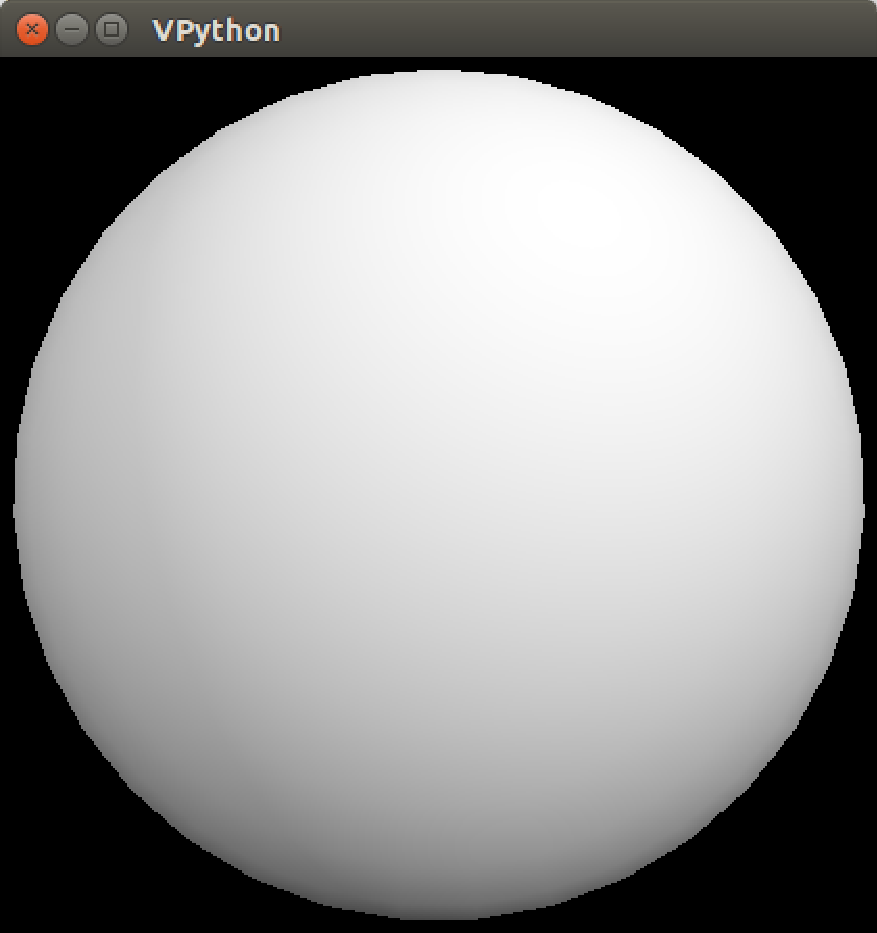
\includegraphics[width=0.2\textwidth]{out/pdf/img/sphere.pdf}
  \end{center}
\end{itemize}
\end{frame}




\iffalse


%%%%%%%%%%%%%%%%% 
\begin{frame}[fragile]
\frametitle{import文}
\begin{itemize}
\item 文法:
\begin{lstlisting}
from @{\bf 名前}@ import *
\end{lstlisting}
\item 効果:
  \begin{itemize}
  \item {\bf 名前}という名前の「モジュール」で提供されている拡張機能
    が使えるようになる
  \end{itemize}
\end{itemize}
\end{frame}

%%%%%%%%%%%%%%%%% 
\begin{frame}[fragile]
\frametitle{import文の例}
\begin{itemize}
\item 例:
\begin{lstlisting}
print cos(0.1)
\end{lstlisting}
\item 出力:
\begin{lstlisting}
Traceback (most recent call last):
  File "a.py", line 1, in <module>
    print cos(0.1)
@\aka{\tt NameError: name 'cos' is not defined}@
\end{lstlisting}
\item 例:
\begin{lstlisting}
from @\aka{math}@ import *  # mathモジュールをimport
print cos(0.1)
\end{lstlisting}
\item 出力:
\begin{lstlisting}
0.995004165278
\end{lstlisting}
\end{itemize}
\end{frame}



%%%%%%%%%%%%%%%%% 
\begin{frame}[fragile]
\frametitle{import文の変形}
\begin{itemize}
\item 文法:
\begin{lstlisting}
import @{\bf 名前}@
\end{lstlisting}
\item 効果:
  \begin{itemize}
  \item {\tt from} {\bf 名前} {\tt import *} と似ているが,
    個々の提供される名前は, 「モジュール名{\tt .}名前」で提供される
  \end{itemize}
\item 
\begin{lstlisting}
import visual
visual.sphere()
\end{lstlisting}
\item こちらの方が面倒だが, 複数のモジュールが同じ名前を
定義していてもOKなので, 「行儀の良い方法」とされる
\end{itemize}
\end{frame}

\fi



%%%%%%%%%%%%%%%%% 
\begin{frame}
\frametitle{ここまでのまとめ}
\begin{itemize}
\item print文 ({\tt print} {\bf 式})
\item 代入文  ({\bf 名前} {\tt =} {\bf 式})
\item 関数定義文 ({\tt def} ...)
\item return文 ({\tt return} {\bf 式})
\item import文 ({\tt import} {\bf 名前}, {\tt import} {\bf 名前} as {\bf 名前}, \ldots)
\item 局所変数の概念
\end{itemize}
\end{frame}


%%%%%%%%%%%%%%%%% 
\begin{frame}
\frametitle{以降}
より様々な,
\begin{itemize}
\item 文
\item データの型(数以外のデータ)
\end{itemize}
に触れる
\end{frame}

%%%%%%%%%%%%%%%%% %%%%%%%%%%%%%%%%% 
\section{for文で繰り返し (1)}
%%%%%%%%%%%%%%%%% %%%%%%%%%%%%%%%%% 

%%%%%%%%%%%%%%%%% 
\begin{frame}[fragile]
\frametitle{for文で繰り返し(1)}
\begin{itemize}
\item 文法 (後に一般化):
\begin{lstlisting}
for @{\bf 名前}@ in range(@{\bf 式}@, @{\bf 式}@):
    @{\bf 文}@
    @{\bf 文}@
    ...
\end{lstlisting}
\item 効果:
\begin{lstlisting}
for @$i$@ in range(@$a$@, @$b$@):
    ...
    ...
\end{lstlisting}
は, $i = a, a+1, \ldots , b-1$に対して, 順に \ldots を実行

\item 補足: {\tt range(式)} は {\tt range(0, 式)} の略記
\end{itemize}
\end{frame}

%%%%%%%%%%%%%%%%% 
\begin{frame}[fragile]
\frametitle{for文で繰り返し(1) : 例1}
\begin{itemize}
\item 
\begin{lstlisting}
for x in range(3, 7):
    print x * x
\end{lstlisting}

\item<2> 出力
\begin{lstlisting}
9
16
25
36
\end{lstlisting}
\end{itemize}
\end{frame}

%%%%%%%%%%%%%%%%% 
\begin{frame}[fragile]
\frametitle{for文で繰り返し(1) : 例2}
\begin{itemize}
\item 
\begin{lstlisting}
def hatena(n):
    a = 1
    for i in range(0, n):
        a = 2 * a + 1
    return a
print hatena(5)
\end{lstlisting}

\item<2> 出力
\begin{lstlisting}
63
\end{lstlisting}
\end{itemize}
\end{frame}


%%%%%%%%%%%%%%%%% 
\begin{frame}[fragile]
\frametitle{for文で繰り返し(1) : 例3}
\begin{itemize}
\item 
\begin{lstlisting}
def hatena(n):
    s = 0
    for i in range(0, n):
        s = s + i * i
    return s
print hatena(8)
\end{lstlisting}

\item<2> 出力
\begin{lstlisting}
140
\end{lstlisting}

\item 
{\scriptsize $0^2 + 1^2 + \cdots + (n-1)^2$を求めよと言われて,
\[ s = s + i * i \]
などという不気味な式を書けるようになることが,
プログラミングに慣れる第一歩なのかも\ldots}

\end{itemize}
\end{frame}



%%%%%%%%%%%%%%%%% 
\begin{frame}[fragile]
\frametitle{if文で場合分け}
\begin{itemize}
\item 文法:
\begin{lstlisting}
if @{\bf 式1}@:
    @{\bf 文}@
    ...
elif: @{\bf 式2}@:
    @{\bf 文}@
    ...
...
else:
    @{\bf 文}@
    ...
\end{lstlisting}
\item elif 以降は省略可. elif は好きな数だけ, else: は最後にひとつ(または無し)
\item 効果:
  \begin{itemize}
  \item まず{\bf 式1}を計算
  \item 結果が偽(0)でなければ最初の選択肢({\bf 文1} ...)を実行
  \item 偽だったら{\bf 式2}を計算
  \item 結果が偽(0)でなければ2番目のの選択肢({\bf 文2} ...)を実行
  \item ...
  \end{itemize}
\end{itemize}
\end{frame}


%%%%%%%%%%%%%%%%% 
\begin{frame}[fragile]
\frametitle{if文で場合分け 例(1)}
\begin{itemize}
\item<1->
\begin{lstlisting}
def one_two_many(x):
    if x == 1:
        return ``ikko''
    elif x == 2:
        return ``niko''
    else:
        return ``takusan''
print one_two_many(2)
print one_two_many(3)
\end{lstlisting}

\item<2> 出力
\begin{lstlisting}
niko
takusan
\end{lstlisting}
\end{itemize}
\end{frame}


%%%%%%%%%%%%%%%%% 
\begin{frame}[fragile]
\frametitle{if文で場合分け 例(2)}
\begin{itemize}
\item<1->
\begin{lstlisting}
def nabetsune():
    for i in range(1, 41):
        if i % 3 == 0 or i % 10 == 3 or 30 < i < 40:
            print i, "!!!!!"
        else:
            print i

nabetsune()
\end{lstlisting}
\item<2>  出力
\begin{lstlisting}
1
2
3 !!!
...
\end{lstlisting}
\end{itemize}
\end{frame}

%%%%%%%%%%%%%%%%% 
\begin{frame}
\frametitle{ここまでとここから}

\begin{center}
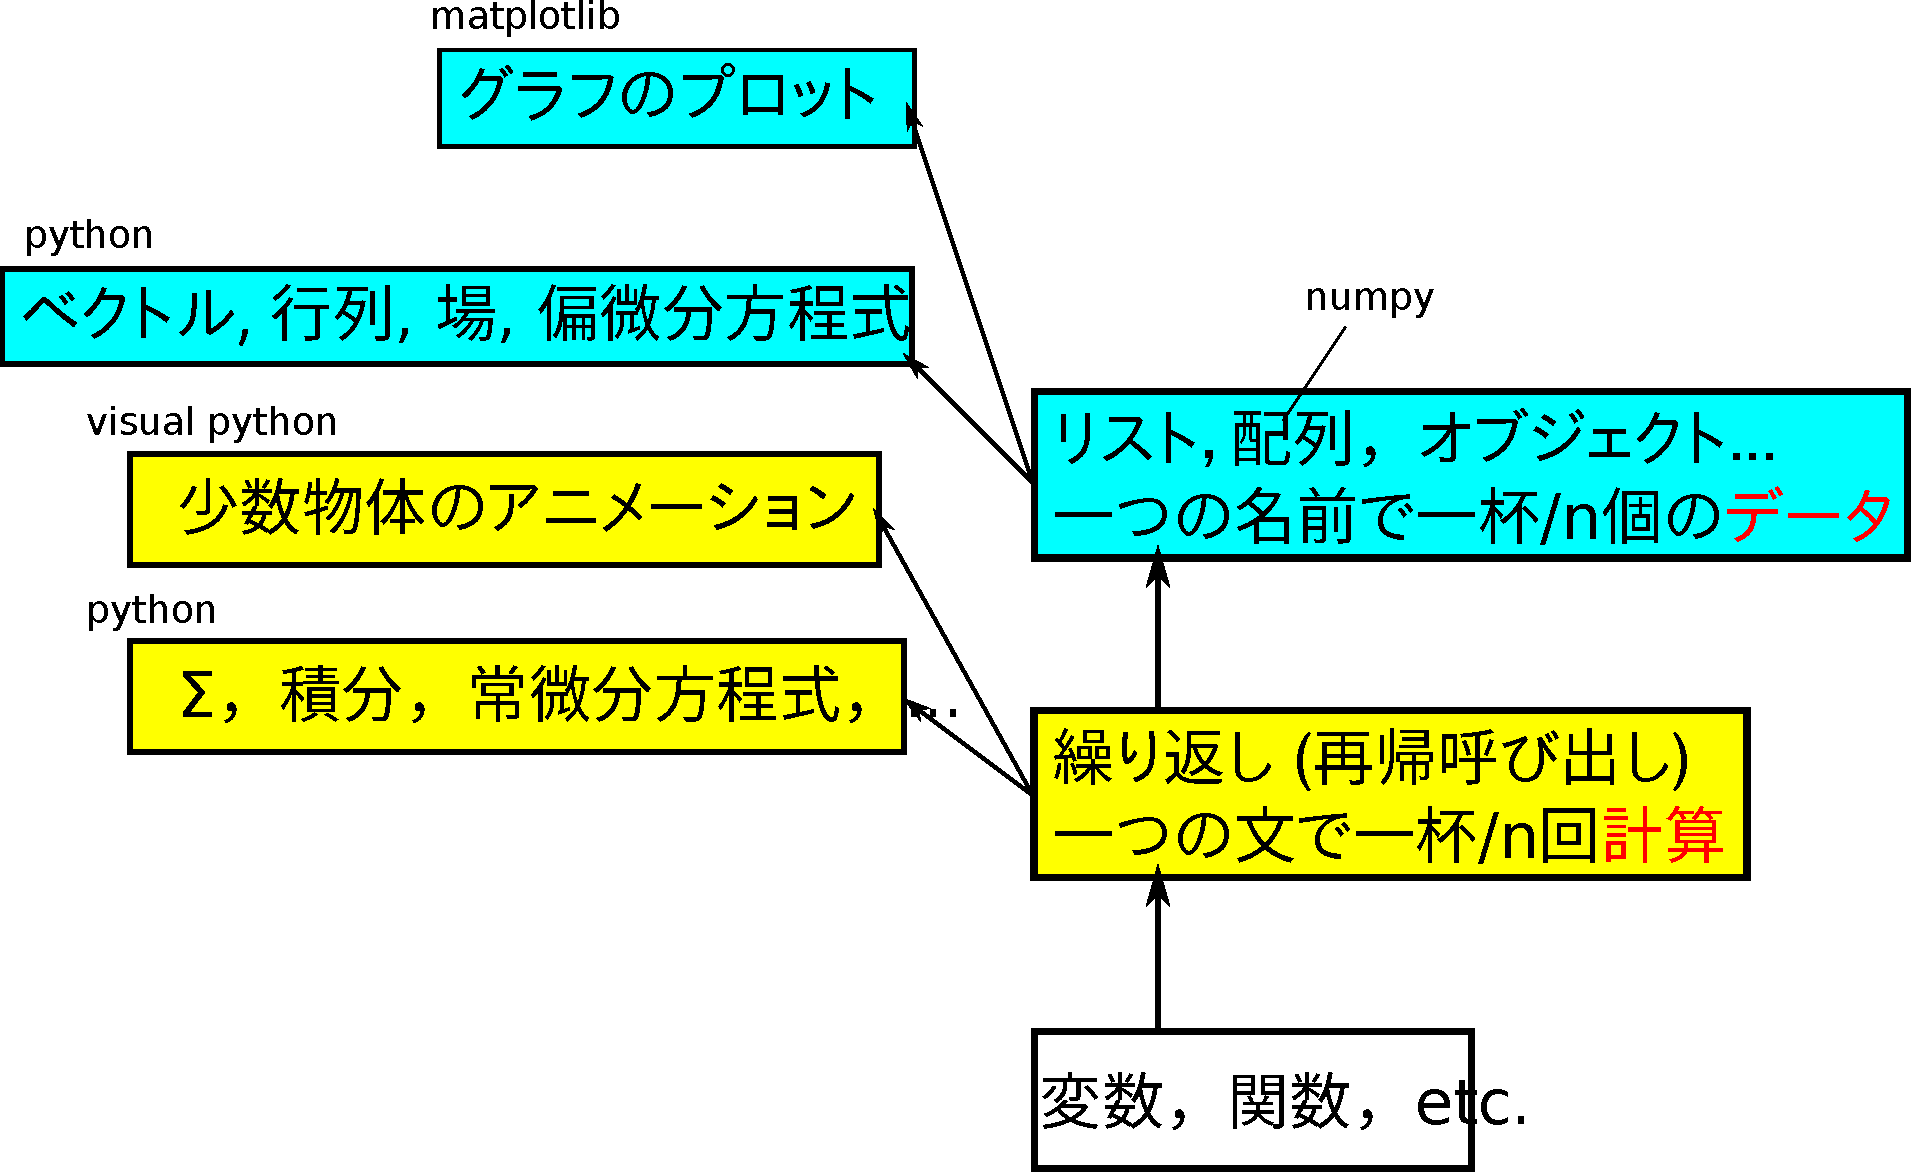
\includegraphics[height=0.9\textheight]{out/pdf/svg/roadmap.pdf}
\end{center}


\end{frame}


%%%%%%%%%%%%%%%%% %%%%%%%%%%%%%%%%% 
\section{より複雑なデータ}
%%%%%%%%%%%%%%%%% %%%%%%%%%%%%%%%%% 

%%%%%%%%%%%%%%%%% 
\begin{frame}[fragile]
\frametitle{より複雑なデータ}
\begin{itemize}
\item これまで, 式の結果として得られる値は基本的には,
ひとつの数値だけだったが
\item 実用的なプログラム(e.g., ベクトル, 行列, 四角, 丸, 果物,
自動車 \ldots)のためには, より複雑な値, 
特に「複数の値を組み合わせた値」が必要
\end{itemize}

\begin{itemize}
\item リスト
\item タプル
\item 文字列
\item 辞書(説明せず)
\item オブジェクト
\end{itemize}

\end{frame}

%%%%%%%%%%%%%%%%% %%%%%%%%%%%%%%%%% 
\section{リスト}
%%%%%%%%%%%%%%%%% %%%%%%%%%%%%%%%%% 

%%%%%%%%%%%%%%%%% 
\begin{frame}[fragile]
\frametitle{リスト}
\begin{itemize}
\item 文法:
\begin{lstlisting}
[ 式, 式, @\ldots@, 式 ]
\end{lstlisting}

\item 意味: 各式を計算した結果を一本に束ねた値(リスト)
\end{itemize}
\end{frame}

%%%%%%%%%%%%%%%%% 
\begin{frame}[fragile]
\frametitle{リスト : 例}
\begin{itemize}
\item 例
\begin{lstlisting}
from math import *
x = 20
a = @\aka{\tt [ 1, 1+2, cos(0.0), x ]}@
print a
print @\aka{len}@(a)    # 要素数
print a@\aka{\tt [}@2@\aka{\tt ]}@      # 特定の要素
b = a @\aka{\tt +}@ [ 1.2, 3.4 ] # 2つのリストつなぐ
print b
c = [ a, a, a ] # リストのリスト
print c[1][2]   # cの1番目の要素(リスト)の2番目の要素
\end{lstlisting}

\item 出力
\begin{lstlisting}
[1, 3, 1.0, 20]
4
1.0
[1, 3, 1.0, 20, 1.2, 3.4]
1.0
\end{lstlisting}

\end{itemize}
\end{frame}

%%%%%%%%%%%%%%%%% 
\begin{frame}[fragile]
\frametitle{リスト : 確認事項}
\begin{itemize}
\item リストも数値と同様, 「値」の一種に過ぎない
\item 数値と同様, 変数に代入したり, 他の関数へ渡したりできる
\item リストを受け取る関数, リストを返す関数, も書ける
\item \ao{「値の種類」が増えたこと以外, 新しいことはない}
\begin{lstlisting}
def f(l):
  return l[0]

print f([1,2,3]) 
\end{lstlisting}
\end{itemize}
\end{frame}


%%%%%%%%%%%%%%%%% 
\begin{frame}[fragile]
\frametitle{リストの書き換え}
リストには, 値を追加・削除したり, 書き換えたりすることができる
\begin{itemize}
\item 
\begin{lstlisting}
a = [ 2, 3, 5 ]
a@\aka{\tt .append}@(7) # 末尾に追加
a[2] = 50
@\aka{\tt del}@ a[1]    # a[1]を削除. 以降の要素は前にずれる
b = [ a, a, a ]
print b
a[2] = 30   # 注目
print b
\end{lstlisting}
\item 
\begin{lstlisting}
[[2, 50, 7], [2, 50, 7], [2, 50, 7]]
[[2, 30, 7], [2, 30, 7], [2, 30, 7]]
\end{lstlisting}
\end{itemize}
\end{frame}


%%%%%%%%%%%%%%%%% 
\begin{frame}[fragile]
\frametitle{リスト内包表記}
\begin{itemize}
\item for文で計算した結果を「一発で」リストにする強力な記法
\item 覚えなくても問題ないが,覚えると賢くなった気がする
\item 文法:
\begin{lstlisting}
[ @\ao{式}@ for 名前 in range(式, 式) ]
\end{lstlisting}
\item この式も, for文同様本当はもっと一般的な文法(後述).

\item 意味: (あたかも「for 名前 in 式」を実行するように
実行し,\ao{式}を計算した結果をリストにする)

\item 例を見たほうが早い
\end{itemize}
\end{frame}


%%%%%%%%%%%%%%%%% 
\begin{frame}[fragile]
\frametitle{リスト内包表記 : 例}
\begin{itemize}
\item 
\begin{lstlisting}
>>> [ x * x for x in range(0, 5) ]
 -> [0, 1, 4, 9, 16]
\end{lstlisting}

\item 
\begin{lstlisting}
>>> sum([ x * x for x in range(0, 5) ])
 -> 30
\end{lstlisting}

% \item 
% \begin{lstlisting}
% >>> X = [ a + (b - a) * i / float(n) for i in range(0, 100000) ]
% >>> sum([ f(x) * (b - a) / float(n) for x in X ]
% \end{lstlisting}
\end{itemize}

それぞれ以下のようにしても同じことだがずっと簡潔
\begin{itemize}
\item 
\begin{lstlisting}
s = []
for x in range(0, 5):
  s.append(x * x)
\end{lstlisting}

\item 
\begin{lstlisting}
s = []
for x in range(0, 5):
  s += x * x
\end{lstlisting}
(注: {\tt s += $E$} は {\tt s = s + $E$}と同じ意味)

% \item 
% \begin{lstlisting}
% >>> X = [ a + (b - a) * i / float(n) for i in range(0, 100000) ]
% >>> sum([ f(x) * (b - a) / float(n) for x in X ]
% \end{lstlisting}
\end{itemize}
\end{frame}


%%%%%%%%%%%%%%%%% %%%%%%%%%%%%%%%%% 
\section{タプル (組)}
%%%%%%%%%%%%%%%%% %%%%%%%%%%%%%%%%% 

%%%%%%%%%%%%%%%%% 
\begin{frame}[fragile]
\frametitle{タプル}
\begin{itemize}
\item 文法:
\begin{lstlisting}
式, 式, @\ldots@, 式
\end{lstlisting}
混乱しないよう, 習慣として括弧をつける
\begin{lstlisting}
(式, 式, @\ldots@, 式)
\end{lstlisting}

\item 意味: 各式を計算した結果を一本に束ねた値
\item リストとほとんど同じ! 実際, 以下はリストと同様に使える
  \begin{itemize}
  \item {\tt len(\ldots)} (要素数)
  \item {\tt \ldots[\ldots]} (指定要素)
  \item {\tt \ldots\ + \ldots} (連結)
  \end{itemize}

\end{itemize}
\end{frame}

%%%%%%%%%%%%%%%%% 
\begin{frame}[fragile]
\frametitle{タプルとリストの違い}
\begin{itemize}
\item タプルは, 一度作ったら要素の追加, 削除, 変更などはできない
\item 
\begin{lstlisting}
a = (1.1, 2.2, 3.3)
a.append(4.4) # @\aka{\tt NG}@
del a[1]      # @\aka{\tt NG}@
a[1] = 22     # @\aka{\tt NG}@
a = (4.4, 5.5) # OK
a = a + (6.6, 7.7) # OK
\end{lstlisting}
\item 最後の2つは, 変数を書き換えているのであってタプルを書き換えている
  のではない
\end{itemize}
\end{frame}

%%%%%%%%%%%%%%%%% 
\begin{frame}[fragile]
\frametitle{タプルの典型的使用場面}
\begin{itemize}
\item 二つ以上の値を一度に返す関数を手軽に書ける
\begin{lstlisting}
def polar(x, y):
    r = sqrt(x * x + y * y)
    theta = atan2(y, x)
    return (r,theta)
\end{lstlisting}
\item 注: {\small 
「二つの値を返す」という言い方はあまり正しくない.
\ao{二つの値を組にした一つの値($=$タプル)}が作れる}

\item 変数に結果を受け取るときもこんなふうに書ける
\begin{lstlisting}
r,theta = polor(3, 4)
\end{lstlisting}

\item 実はこれでも「なぜリストだけじゃダメ?」の答えにはなっていないが
  \begin{itemize}
  \item ちなみにこれもOK
\begin{lstlisting}
[a0,a1,a2] = range(3,6)  # a0=3, a1=4, a2=5
\end{lstlisting}
\end{itemize}

\end{itemize}
\end{frame}


%%%%%%%%%%%%%%%%% %%%%%%%%%%%%%%%%% 
\section{文字列}
%%%%%%%%%%%%%%%%% %%%%%%%%%%%%%%%%% 

%%%%%%%%%%%%%%%%% 
\begin{frame}[fragile]
\frametitle{文字列}
\begin{itemize}
\item 文法:
\begin{lstlisting}
"文字文字 @\ldots@ 文字"
'文字文字 @\ldots@ 文字'
"""文字文字 @\ldots@ 文字"""
'''文字文字 @\ldots@ 文字'''
\end{lstlisting}

\item どれもほとんど同じ意味. なぜ色々ある?
  \begin{itemize}
  \item 文字列中に{\tt "}を含めたければ, {\tt '}が便利. 逆もまた然り
    \begin{itemize}
    \item {\tt a = 'he greeted, "hi"'}
    \item {\tt b = "Obama's lecture"}
    \end{itemize}
  \item 3連打({\tt """}, {\tt '''})は, 改行を含んでも良い
  \end{itemize}

\item そして, できる操作はまたしてもリストやタプルとそっくり
  \begin{itemize}
  \item {\tt len(\ldots)}
  \item {\tt \ldots[\ldots]}
  \item {\tt \ldots\ + \ldots}
  \end{itemize}
\end{itemize}
\end{frame}

%%%%%%%%%%%%%%%%% 
\begin{frame}[fragile]
\frametitle{文字列特有の操作: 値の埋め込み}
\begin{itemize}
\item (例えば)ある変数xの値を表示したい場合,
\begin{lstlisting}
print x    
\end{lstlisting}
\item でもよいが, すぐに何がどこで表示されたのかわからなくなる.
もっとわかりやすく,
\begin{lstlisting}
print "x = %s" % x
\end{lstlisting}
のようにする

\item 例
\begin{lstlisting}
from math import *
y = cos(3.14)
print "cos(3.14) = %s" % y
\end{lstlisting}
\end{itemize}
\end{frame}

%%%%%%%%%%%%%%%%% 
\begin{frame}[fragile]
\frametitle{文字列への値の埋め込み : 2つ以上の値}
\begin{itemize}
\item 2つ以上の値を埋め込みたければ, {\tt \%}の右にタプルを書く
\item 例
\begin{lstlisting}
from math import *
x = 2.3
print "cos(%s) = %s" % (x, exp(x))
\end{lstlisting}
\end{itemize}
\end{frame}

%%%%%%%%%%%%%%%%% 
\begin{frame}[fragile]
\frametitle{文字列への値の埋め込み : 規則}

\begin{itemize}
\item 一般に,
\begin{lstlisting}
式1 % 式2
\end{lstlisting}
において, 式1の結果が文字列だったら, 
上記の結果は式1中の左から$i$番目の{\tt \%s}を, 
式2の結果の第$i$番目の要素で置き換えた文字列

\item {\tt \%s}以外に, 表示したいデータの種類により,
色々あるがとりあえず{\tt \%s}は汎用的なのでこれを覚えれば良い
\item 一応\ldots
  \begin{itemize}
  \item {\tt \%d} : 整数
  \item {\tt \%9d} : 整数. ただし9文字以下は9文字分の幅になるよう右揃え
  \item {\tt \%f} : 浮動小数点数
  \item {\tt \%.3f} : 浮動小数点数. ただし, 小数点以下3桁まで
  \item など
  \end{itemize}
\end{itemize}
\end{frame}


%%%%%%%%%%%%%%%%% 
\begin{frame}[fragile]
\frametitle{このゼミでのリスト・タプル・文字列の重要性 (1)}
\begin{itemize}
\item Python一般ににおいてはかなり重要な機能
\item ベクトルや行列をつくろうと思ったら,
  普通はこれらを使いこなすことになる
\item が, このゼミではベクトルや行列は, 
  もっとすごいの(visualのvector, 
  numpyの多次元配列)を使うことを主眼にしているので,
  あまり深入りせずに先へ進む
\end{itemize}

より詳しい説明は
\hyperlink{https://docs.python.jp/3.5/tutorial/index.html}
{Pythonチュートリアル}5章「データ構造」を参照
\end{frame}

%%%%%%%%%%%%%%%%% 
\begin{frame}[fragile]
\frametitle{このゼミでのリスト・タプル・文字列の重要性 (2)}
\begin{itemize}
\item Pythonでは, \ao{実は異なるものが表面上同じ書き方で書け,}
  実際それが貫かれている, 
  という設計思想(オブジェクト指向, 多態性)に馴染むことも重要
  \begin{itemize}
  \item リスト, タプル, 文字列どれにも, 
    {\tt +, len, [\ldots]}などが適用可能
  \item numpyの多次元配列やVisual Pythonのvectorもそれらと似ている
  \end{itemize}
\item 全く同じではないところが時に混乱の元となる
\item 「色々あるのだがそれらが似た表記で使えるように,
  縁の下で頑張っている」という点を理解しておく
\end{itemize}
\end{frame}


%%%%%%%%%%%%%%%%% 
\begin{frame}[fragile]
\frametitle{for文で繰り返し(2)}
\begin{itemize}
\item これまでfor文は以下の形であると言ってきた
\begin{lstlisting}
for @{\bf 名前}@ in @{\tt range(\aka{\bf 式, 式})}@:
    @{\bf 文}@
    @{\bf 文}@
    ...
\end{lstlisting}
\item 実はより一般的:
\begin{lstlisting}
for @{\bf 名前}@ in @\aka{\bf 式}@:
    @{\bf 文}@
    @{\bf 文}@
    ...
\end{lstlisting}
\item ここで, \aka{\bf 式}には, 
  {\tt range($a$, $b$)}だけでなく,
  リスト, タプル, 文字列など,
  色々なものが来れる
\item 実は, 
  {\tt range($a$, $b$)}は{\tt [ $a$, $a+1$, \ldots $b-1$ ]}
  というリストを作る関数に過ぎなかった
\end{itemize}
\end{frame}

%%%%%%%%%%%%%%%%% 
\begin{frame}[fragile]
\frametitle{for文で繰り返し(2)}
\begin{itemize}
\item 例:
\begin{lstlisting}
for x in [ 2, 3, 5 ]:
    print x
for x in "hello":
    print x
\end{lstlisting}
\item 
\begin{lstlisting}
2
3
5
h
e
l
l
o
\end{lstlisting}
\end{itemize}
\end{frame}


%%%%%%%%%%%%%%%%% 
\begin{frame}[fragile]
\frametitle{for文で繰り返し(2)}
\begin{itemize}
\item リストの各要素がタプルの場合はこんな書き方も許される
\begin{lstlisting}
A = [ (0,1), (2,3), (4, 5) ]
for @\aka{\tt x,y}@ in A:
    print x + y
\end{lstlisting}

\item 出力
\begin{lstlisting}
1
5
9
\end{lstlisting}

\item 以下のような文が許されることの拡張と思えば自然
\begin{lstlisting}
x,y = タプル
\end{lstlisting}
\end{itemize}
\end{frame}


%%%%%%%%%%%%%%%%% 
\begin{frame}[fragile]
\frametitle{for文で繰り返し(2) : zip}
\begin{itemize}
\item \ao{\tt zip($X$, $Y$)}という関数で二つの同じ長さのリストを,タプルのリストにできる
\item 二つのリストからひとつずつ要素を取り出すような処理をfor文で書くのに重宝する
\begin{lstlisting}
X = [ 1, 2, 3 ]
Y = [ 1, 4, 9 ]
print zip(X, Y)
for @\aka{\tt x,y}@ in zip(X, Y):
    print x + y
\end{lstlisting}

\item 出力
\begin{lstlisting}
[ (1,1), (2,4), (3,9) ]
2
6
12
\end{lstlisting}
\end{itemize}
\end{frame}

%%%%%%%%%%%%%%%%% 
\begin{frame}[fragile]
\frametitle{for文で繰り返し(2) : enumerate}
\begin{itemize}
\item \ao{\tt enumerate($L$)} という関数で,リストの各要素を,
そのインデクス(リスト内での位置; 0, 1, 2, \ldots)とともに処理できる
\item リスト内の出現位置を返したい場合や,出現位置が計算結果に意味を持つ場合に有用
\begin{lstlisting}
def find_space():
  for @\aka{\tt i,c}@ in enumerate("hello world"):
    if c == ' ':
      return i
  return -1
\end{lstlisting}

\item 出力
\begin{lstlisting}
5
\end{lstlisting}
\end{itemize}
\end{frame}


%%%%%%%%%%%%%%%%% %%%%%%%%%%%%%%%%% 
\section{その他の制御構文}
%%%%%%%%%%%%%%%%% %%%%%%%%%%%%%%%%% 

\begin{frame}
\frametitle{その他の構文}

\begin{itemize}
%\item \aka{if文} : 条件によって異なる文を実行
\item \aka{while文} : 条件が成り立つ限り繰り返し(for文より一般的な繰り返し)
\item \aka{break文} : for, whileを好きな時点で強制終了
\item \aka{continue文} : for, whileの「一回の繰り返し」を終了
  (次の繰り返しへ進む)
\end{itemize}

グダグダ説明するのを省略して, 
\hyperlink{https://docs.python.jp/3.5/tutorial/index.html}
{Pythonチュートリアル}第4章 「その他の制御フルーツール」を参照

\end{frame}





%%%%%%%%%%%%%%%%% %%%%%%%%%%%%%%%%% 
\section{クラスとオブジェクト}
%%%%%%%%%%%%%%%%% %%%%%%%%%%%%%%%%% 
\begin{frame}
\frametitle{オブジェクト}
\begin{itemize}
\item オブジェクト : 言葉通り「もの」
\item Pythonにおいては, \ao{色々な属性をひとまとめにした値}
\item たとえば, 
  \begin{itemize}
  \item 「球」は「中心」と「半径」
  \item 「複素数」は「実部」と「虚部」
  \item 「野球チーム」は「監督」と「選手のリスト」
  \item etc.
  \end{itemize}
\item 新しい種類(class)のオブジェクトを自分で定義することもできるが,
ここでは説明しない
\end{itemize}
\end{frame}


%%%%%%%%%%%%%%%%% %%%%%%%%%%%%%%%%% 
\begin{frame}[fragile]
\frametitle{オブジェクトについて知っておくべき最低限の事(1)}

\begin{itemize}
\item みんなみんな実はオブジェクト
  \begin{itemize}
  \item Visual Pythonのvector, sphere, arrow, \ldots
  \item (これから出る) numpyの「配列」
  \item 実はリストやタプルもオブジェクト
  \end{itemize}
\item オブジェクトに対してできること
  \begin{enumerate}
  \item メソッド($\approx$関数を呼び出す) 
\begin{lstlisting}
a.append(x)
\end{lstlisting}
  \item 属性(フィールド)に値をセット 
\begin{lstlisting}
c.pos = vector(1,2,3)
\end{lstlisting}
  \item 属性を参照 c.x
\begin{lstlisting}
print c.x
\end{lstlisting}
\end{enumerate}
\end{itemize}
\end{frame}


%%%%%%%%%%%%%%%%% %%%%%%%%%%%%%%%%% 

\begin{frame}[fragile]
\frametitle{クラスとオブジェクト: 本当に最小の例}
\begin{itemize}
\item 仕組みについて詳細に知る必要はない
\item vector, sphere, なども「どこかで」
  こんな風に定義されている,とだけ心に留めとけばよし
\item []
\begin{lstlisting}
class nothing:
    pass  # 何もしない
# nothingクラスのオブジェクトを作る
m = nothing()
# 属性値へ代入(@$\approx$@変数への代入)
m.x = 10
m.y = 20
# 属性値を参照
print m.x + m.y
# もちろんオブジェクトを入力に取る関数も書ける
def take_nothing(n):
    n.x = n.x + 100

take_nothing(m)
print m.x
\end{lstlisting}
\end{itemize}
\end{frame}

%%%%%%%%%%%%%%%%% %%%%%%%%%%%%%%%%% 
\begin{frame}
\frametitle{オブジェクトについて知っておくべき最低限の事(2)}
\begin{itemize}
\item オブジェクトには「種類(vector, リスト, タプル, ...)」
がある $=$ ある\ao{クラス}に属している
\item \ao{同じ名前のメソッドでも, クラスが異なれば動作(定義)が異なる}
\item \ao{$a$ {\tt +} $b$とか,普段何気なくやっている動作も,}
  クラスが異なれば動作が異なる
\item これは
  \begin{enumerate}
  \item 便利で強力 (数学でも{\tt +}は数, ベクトル, 行列, etc.
    で定義が異なるが名前は同じ)
  \item 一方,ちゃんと意識しないと混乱や理解を曖昧にするもと
  \end{enumerate}
\item 多くの場合その名前にふさわしい「自然な」動作が定義されていると
期待する一方で,それらが「ひとりでに」「書き手の意図を読んで」
行われるわけでは決して無いことを理解しよう
\end{itemize}
\end{frame}

%%%%%%%%%%%%%%%%% %%%%%%%%%%%%%%%%% 
\begin{frame}[fragile]
\frametitle{同じメソッドの名前でも, classが異なれば動作が異なる}
\begin{itemize}
\item 例: {\tt append}
\begin{lstlisting}
import random
from visual import *
def rnd():
    return random.random()
l = @\ao{\tt []}@
c = @\ao{\tt curve()}@
for i in range(10):
    l.append(vector(rnd(), rnd(), rnd()))
for i in range(10):
    c.append(vector(rnd(), rnd(), rnd()))
\end{lstlisting}
\end{itemize}
\end{frame}


%%%%%%%%%%%%%%%%% %%%%%%%%%%%%%%%%% 
\begin{frame}[fragile]
\frametitle{{\tt +}でさえも}
\begin{itemize}
\item<1-> []
\begin{lstlisting}
from visual import *  # vector
import numpy as np    # array
print 1 @\ao{\tt +}@ 2
print [1,2,3] @\ao{\tt +}@ [4,5,6]
print vector(1,2,3) @\ao{\tt +}@ vector(4,5,6)
print np.array([1,2,3]) @\ao{\tt +}@ np.array([4,5,6])
\end{lstlisting}

\item<2-> []
\begin{lstlisting}
3
[1,2,3,4,5,6]
<5, 7, 9>
[5 7 9]
\end{lstlisting}
\end{itemize}
\end{frame}

%%%%%%%%%%%%%%%%% %%%%%%%%%%%%%%%%% 
\begin{frame}[fragile]
\frametitle{{\tt *}も}
\begin{itemize}
\item<1-> []
\begin{lstlisting}
from visual import *  # vector
import numpy as np    # array
print 3 @\ao{\tt *}@ 4
print [1,2,3] @\ao{\tt *}@ 5
print vector(1,2,3) @\ao{\tt *}@ 10
print 100 @\ao{\tt *}@ vector(1,2,3)
print np.array([1,2,3]) @\ao{\tt *}@ 1000
print 10000 @\ao{\tt *}@ np.array([1,2,3])
\end{lstlisting}
\item<2-> []
\begin{lstlisting}
12
[1,2,3,1,2,3,1,2,3,1,2,3,1,2,3]
<10, 20, 30>
<100, 200, 300>
[1000 2000 3000]
[10000 20000 30000]
\end{lstlisting}
\end{itemize}
\end{frame}


%%%%%%%%%%%%%%%%% %%%%%%%%%%%%%%%%% 
\begin{frame}[fragile]
\frametitle{もちろん{\tt **}も}
\begin{itemize}
\item<1-> []
\begin{lstlisting}
from visual import *  # vector
import numpy as np    # array
print 3 @\ao{\tt **}@ 4
print [1,2,3] @\ao{\tt **}@ 20
print vector(1,2,3) @\ao{\tt **}@ 100
print np.array([1,2,3]) @\ao{\tt **}@ 4 
\end{lstlisting}
\item<2-> []
\begin{lstlisting}
81
# エラー
# エラー
[ 1 16 81]
\end{lstlisting}
\end{itemize}
\end{frame}

\iffalse

%%%%%%%%%%%%%%%%% %%%%%%%%%%%%%%%%% 
\begin{frame}[fragile]
\frametitle{クラス}
\begin{itemize}
\item オブジェクトを生み出す「ひな形」「設計図」
\item 文法:
\begin{lstlisting}
class クラス名:
    関数定義
    関数定義
    ...
\end{lstlisting}
\item 効果:
  \begin{itemize}
  \item 「クラス名」で関数(コンストラクタ)が定義され, 
    呼び出されると新しいオブジェクトが作られる
  \item オブジェクトには属性値を代入できる
  \end{itemize}
\end{itemize}
\end{frame}

%%%%%%%%%%%%%%%%% %%%%%%%%%%%%%%%%% 
\begin{frame}[fragile]
\frametitle{クラスとオブジェクト: もう少しそれらしい例}

\begin{itemize}
\item \aka{\tt \_\_init\_\_}という関数で,
コンストラクタの中身を定義できる
\item その他好きな名前で関数(\aka{メソッド})を定義できる
\item メソッドの第一引数は作られたオブジェクトが渡される
  (普通\aka{\tt self}という変数名を使う)
\item 
\begin{lstlisting}
class baseball_team:
    # コンストラクタが呼び出されるとこれが呼び出される
    def @\aka{\tt \_\_init\_\_}@(@\aka{\tt self}@, name, manager, players):
        self.name = name
        self.manager = manager
        self.players = players
    # メソッドの定義
    def add_player(@\aka{\tt self}@, p):
        self.players.append(p)
\end{lstlisting}
\end{itemize}
\end{frame}

%%%%%%%%%%%%%%%%% %%%%%%%%%%%%%%%%% 
\begin{frame}[fragile]
\frametitle{クラスとオブジェクト: もう少しそれらしい例}
\begin{itemize}
\item<1-> 
\begin{lstlisting}
# オブジェクト作成 -> コンストラクタ__init__呼び出し
r = @\aka{\tt baseball\_team}@("Nipponham", "Kuriyama", 
                  [ "Inaba", "Saito", "Takeda" ])
print r.players
# メソッド呼び出し
@\aka{\tt r.add\_player}@("Ohtani")
print r.players
\end{lstlisting}

\item<2->
\begin{lstlisting}
[ "Inaba", "Saito", "Takeda" ]
[ "Inaba", "Saito", "Takeda", "Ohtani" ]
\end{lstlisting}
\end{itemize}

\end{frame}

%%%%%%%%%%%%%%%%% %%%%%%%%%%%%%%%%% 
\begin{frame}[fragile]
\frametitle{このゼミと, クラス・オブジェクト}
\begin{itemize}
\item 大きなプログラムを作るのにクラス・オブジェクトは非常に重要
\item このゼミでは, 
  自らクラス・オブジェクトを作る必要はあまりない
\item 一方, Visual Python, numpy を始め, 提供される機能は大部分が,
  オブジェクトとして提供されるため, 「どんな風に使うか」はマスターする
  必要あり(メソッドを呼ぶ, 属性値を参照・変更する)
\item 以下の例でもオブジェクトをいくつも作っている
  ({\tt vector}, {\tt sphere}, {\tt +}いずれもオブジェクトを返す)
\begin{lstlisting}
center = vector(2, 3, 4)
s = sphere(pos=center)
s.pos = center + vector(1, 1, 1)
\end{lstlisting}
\end{itemize}

% クラス・オブジェクトのもう少し丁寧な説明は,
% \hyperlink{http://www.physics.orst.edu/~rubin/Books/eBookWorking/index.html}{教科書SOCP}の 4.4
% ABSTRACT DATA STRUCTURES, OBJECTS (CS) を参照

\end{frame}

%%%%%%%%%%%%%%%%% %%%%%%%%%%%%%%%%% 
\begin{frame}[fragile]
\frametitle{特別なメソッド}
\begin{itemize}
\item 例えば{\tt \_\_add\_\_(self, o)}
というメソッドを定義すると, 足し算({\tt +})を定義できる
\item {\tt x + y}は, {\tt x.\_\_add\_\_(y)}の意味

\begin{lstlisting}
class vector:
  def @\aka{\tt \_\_init\_\_}@(self, x, y, z):
    self.x = x
    self.y = y
    self.z = z
  def @\aka{\tt \_\_add\_\_}@(self, o):
    return vector(self.x + o.x, self.y + o.y, 
                  self.z + o.z)

u = vector(1,2,3)
v = u + vector(4, 5, 6) # u.__add__(vector(4, 5, 6))
print v
\end{lstlisting}

\item 他にも, {\tt \_\_sub\_\_}, {\tt \_\_mul\_\_}, {\tt \_\_div\_\_}など
\end{itemize}
\end{frame}

%%%%%%%%%%%%%%%%% %%%%%%%%%%%%%%%%% 
\begin{frame}[fragile]
\frametitle{特別なメソッド}

\begin{itemize}
\item Pythonではこうして, {\tt +}, {\tt -}, {\tt *}など,
  \ao{馴染みの記法で, オブジェクトに相応しい動作}
  を行わせることができる
\item Pythonのリスト, タプル(\ao{連結}), 
  Visual Pythonのvector (\ao{ベクトルの和}), numpyのarray, matなど
\item それらの動作は通常, 自然なためあまり意識することは無いが,
  決して人間のように「文脈から」「空気から」
  判断しているわけではないので注意
\item 例えば, vectorとリストをごっちゃにすると, 
  {\tt +}の動作の違いであたふたすることになる
\end{itemize}
\end{frame}

%%%%%%%%%%%%%%%%% %%%%%%%%%%%%%%%%% 
\section{Visual Python ステップ2}
%%%%%%%%%%%%%%%%% %%%%%%%%%%%%%%%%% 


%%%%%%%%%%%%%%%%% %%%%%%%%%%%%%%%%% 
\begin{frame}[fragile]
\frametitle{Visual Pythonプログラム例を改めて鑑賞}
\begin{lstlisting}
from visual import *
s1 = sphere(color=color.red) # キーワード引数
s2 = sphere(pos=@\aka{\tt vector(1.0, 2.0, 3.0)}@, radius=0.1)
# s1, s2はオブジェクト
rate(0.3) # 約3.3秒待つ (0.3フレーム/秒)
# 属性へ代入
s2.color = color.green  # 色が緑に変わる
rate(0.3) # 約3.3秒待つ (0.3フレーム/秒)
s2.pos = s2.pos @\aka{\tt +}@ 0.5 @\aka{\tt *}@ vector(-1.0,-1.0,-1.0) # 球が「動く」
\end{lstlisting}

\begin{itemize}
\item Visual Pythonの\ao{vectorで3次元ベクトル}を作れる
\item \ao{{\tt +} はベクトルの足し算, {\tt *}はスカラー倍}
  という自然な動作をする
\end{itemize}
\end{frame}

\fi

%%%%%%%%%%%%%%%%% %%%%%%%%%%%%%%%%% 
\begin{frame}[fragile]
\frametitle{Visual Pythonのvector}
\begin{itemize}
\item [] 3次元ベクトルに特化したデータ
\item []
\begin{lstlisting}
>>> from visual import *
>>> v = vector(1,2,3)
>>> v
vector(1, 2, 3)
>>> @\ao{\tt dir}@(v)  # オブジェクトのフィールドやメソッドを探る
[ ..., 'astuple', 'clear', 'comp', 'cross', 'diff_angle', 'dot', 'mag', 'mag2', 'norm', 'proj', 'rotate', 'x', 'y', 'z']
>>> v.x
1
>>> v[0]  # v.xと同じこと. お好きな方をどうぞ
1
\end{lstlisting}
\end{itemize}
\end{frame}


%%%%%%%%%%%%%%%%% %%%%%%%%%%%%%%%%% 
\begin{frame}[fragile]
\frametitle{Visual Pythonのvector}
\begin{itemize}
\item その他のありがたい機能
\item []
\begin{lstlisting}
>>> v@\ao{\tt .mag}@    # |v|
3.7416573867739413
>>> v@\ao{\tt .mag2}@   # |v|^2
14.0
>>> v@\ao{\tt .dot}@(v) # v と v の内積
14.0
>>> v@\ao{\tt .norm}@() # 単位ベクトル化
vector(0.267261241912424, 0.534522483824849, 0.801783725737273)
>>> v.mag * v.norm()
vector(1, 2, 3)
>>> v@\ao{\tt .cross}@(vector(1,1,1)) # 外積
vector(-1, 2, -1)
\end{lstlisting}
\end{itemize}
\end{frame}

\iffalse

%%%%%%%%%%%%%%%%% %%%%%%%%%%%%%%%%% 
\begin{frame}[fragile]
\frametitle{Visual Pythonプログラム例を改めて鑑賞}
\begin{lstlisting}
from visual import *
s1 = sphere(color=color.red) # キーワード引数
s2 = sphere(pos=vector(1.0, 2.0, 3.0), radius=0.1)
# s1, s2はオブジェクト
@\aka{\tt rate(0.3)}@ # 約3.3秒待つ (0.3フレーム/秒)
# 属性へ代入
s2.color = color.green  # 色が緑に変わる
@\aka{\tt rate(0.3)}@ # 約3.3秒待つ (0.3フレーム/秒)
s2.pos = s2.pos + 0.5 * vector(-1.0,-1.0,-1.0) # 球が「動く」
\end{lstlisting}

\begin{itemize}
\item Visual Pythonの\ao{\tt rate($f$)}関数は, 画面の更新と,
  $f$フレーム/秒になるような時間調節 ($\approx 1/f$秒休む)
\item \aka{rateを呼ばないと}
画面の更新がないまま計算が進行し, 
最終状態だけが表示される\aka{(アニメーションにならない)}ので注意
\end{itemize}
\end{frame}

\fi


%%%%%%%%%%%%%%%%% %%%%%%%%%%%%%%%%% 
\begin{frame}[fragile]
\frametitle{プログラム中のコメント}
\begin{itemize}
\item プログラム中に注釈(コメント)を書くことは,
実はすごく重要
\item Pythonでは, 各行\aka{{\tt \#}以降}がコメント
\begin{lstlisting}
def main():
    @\aka{\tt \# location of the pointmass}@
    p = vector(1,2,3)
    @\aka{\tt \# the pointmass}@
    s = sphere(pos=p)
    @\aka{\tt \# the spring}@
    sp = helix(pos=p)
    ...
\end{lstlisting}

\item 日本語で書きたい場合,
ファイルの1行目に以下を書いておく
\begin{lstlisting}
@\aka{\tt \#! -*- coding: utf-8 -*-}@
\end{lstlisting}
\end{itemize}

\end{frame}


\end{document}
